\chapter{Konzeption und Aufbau des Prototyps}\label{sec:concept}
Nachdem in der Literaturrecherche (Kapitel \ref{sec:related-works}) zentrale funktionale und gestalterische Anforderungen identifiziert und in Kapitel \ref{sec:analysis} vergleichbare Spiele hinsichtlich ihres Game- und Rätseldesigns analysiert wurden, kann \say{Connecting-Minds} nun auf Basis dieser Erkenntnisse vollständig konzipiert werden. Ergänzend fließt die von \cite{krekhov_puzzles_2021} entwickelte Taxonomie für analoge und digitale Escape-Room-Spiele in den Gestaltungsprozess mit ein.

Die Konzeption des Spiels folgt einem systematisch-methodischen Vorgehen. Zunächst werden die übergeordneten Designvision sowie die grundlegenden Zielsetzungen erläutert. Darauf aufbauend dient das \ac{MDA}-Framework (vgl. \citealp{hunicke_mda_2004}) als zentrales Analyse- und Strukturierungsinstrument, um die angestrebte Spielerfahrung gezielt gestalten zu können. In diesem Rahmen werden die grundlegenden Spielmechaniken, die Rollenverteilung sowie die angestrebten dynamischen Prozesse beschriben. Im Anschluss folgen die Darstellung der technischen Verbundenheit der Anwendungen, das Konzept für das Tutorial, Überlegungen zum Dialog- und Sounddesign sowie eine abschließende Reflexion über die Ideen und Ansätze, die im finalen Prototyp keine Berücksichtigung mehr gefunden haben.

\section{Designziele und Zielgruppe}
\say{Connecting-Minds} verfolgt das Ziel, kooperative Kommunikation unter asymmetrischen Perspektiven in einem Escape-Room-ähnlichen Szenario zu fördern. Das Spiel basiert auf der Zusammenarbeit zweier Rollen, Player und Watcher, die gemeinsam Rätsel lösen und Hindernisse in der Spielwelt überwinden müssen. Beide Rollen verfügen über unterschiedliche Wahrnehmungen und Interaktionsmöglichkeiten innerhalb der Spielwelt, die sich gegenseitig ergänzen und auf Kooperation angewiesen sind.

Das Spiel lässt sich dem Genre der kooperativen Adventure-Spiele zuordnen.

Im Zentrum des spielerischen Erlebnisses steht die gezielte Verteilung asymmetrischer Informationen, um eine Balance zwischen Orientierung und Vertrauen zu schaffen. Der gemeinsame Fortschritt bildet dabei den zentralen Motivationsfaktor.

Die Zielgruppe entspricht derjenigen, die bereits in der vorangegangenen Konzeptionsphase im Rahmen des Moduls \textit{Interaktionsdesign} im \ac{UCD}-Prozess entwickelt wurde. Im Fokus stehen drei exemplarische Personae:

\begin{itemize}
    \item \textbf{Steve Works}, 19 Jahre alt, ist Studienganganfänger im Fach Medieninformatik. Neben seinem akademischen Interesse sucht er gezielt nach sozialer Interaktion. Spieleabende und gemeinschaftliche Aktivitäten betrachtet er als Möglichkeit, Kontakte zu knüpfen und den Studienalltag aktiv zu gestalten.
    \item \textbf{Uwe Kaufmann}, 64 Jahre alt, ist erfahrener Projektleiter. Er steht vor der Aufgabe, ein neues Team zusammenzustellen und sieht in \say{Connecting-Minds} eine Gelegenheit, Teambuilding und Motivation zu fördern, um eine effektive Zusammenarbeit zu etablieren.
    \item \textbf{Anja Gayms}, 31 Jahre alt, arbeitet als introvertierte Zahnarzthelferin. Sie sucht im Spiel sowohl eine kognitive Herausforderung als auch eine Gelegenheit, bestehende Freundschaften zu vertiefen.
\end{itemize}

Die vollständige Ausarbeitung der Personae befinden sich im Anhang \ref{sec:append_concept_personae}: \nameref{sec:append_concept_personae}.

\section{Narratives und funktionales Grundgerüst}
Das Spiel basiert auf einem asymmetrischen Zwei-Rollen-Prinzip, bei dem zwei Spieler unterschiedliche Rollen einnehmen und gemeinsam innerhalb einer geteilten Spielwelt agieren. Diese Welt ist in mehrere räumlich und funktional voneinander abgegrenzte Abschnitte gegliedert. Der Fortschritt im Spiel wird durch kooperatives Handeln und das gemeinsame Lösen von Rätsel ermöglicht. Dabei ist die wechselseitige Abhängigkeit beider Rollen wesentlich für das Vorankommen.

Die narrative Struktur des Spiels entfaltet sich durch eine Kombination aus textbasierten Hinweisen, Umweltinformationen und der räumlichen Gestaltung. Das Storytelling ist dabei stark an das sog. \say{Environmental Storytelling} angelehnt, bei dem die Umgebung selbst narrative Funktionen übernimmt.

Die zugrundeliegende Hintergrundgeschichte lautet wie folgt:

Der Protagonist des Spiels nimmt man einer experimentellen Simulation innerhalb seines Forschungsinstituts teil. Diese Simulation verläuft jedoch nicht wie geplant. Durch eine unerwartete Anomalie während des Prozesses wird das Selbst des Protagonisten gespalten. Zurück bleibt der physische Körper in der realen Welt, während das Bewusstsein in das digitale Netz der Forschungseinrichtung übertragen wird. Beide Entitäten, Körper und Geist, existieren fortan getrennt, können jedoch auf bislang unerklärliche Weise miteinander kommunizieren. Ziel beider Instanzen ist es, die Ursache der Anomalie zu ergründen, den oder die Verantwortlichen ausfindig zu machen und schließlich die eigene Wiedervereinigung herbeiführen.

Die Spielwelt bildet diesen narrativen Rahmen architektonisch und funktional ab. Beginnend in einem alten, unterirdischen Gewölbe des Forschungsinstituts, in das der leibliche Körper nach dem fehlgeschlagenen Experiment gebracht wurde, arbeiten sich die beiden Rollen durch verschiedene Abteilungen der Einrichtung. Dabei sammeln sie Hinweise auf die Hintergründe des Vorfalls und identifizieren mögliche Antagonisten. Im weiteren Verlauf öffnet sich die Spielwelt sukzessive. Sie führt zunächst durch unterschiedliche Gebäudeteile der Forschungseinrichtung, anschließend in Außenareale sowie in die privaten Wohnräume von Personen, die in den Vorfall verwickelt sein könnten. Die Erweiterung der Spielwelt entsteht dabei stets im direkten Zusammenhang mit dem narrativen Fortschritt.


\section{Spielkonzeption mithilfe des MDA-Frameworks}
% Aus den bisherigen Forschungen zum Thema asymmetrischen kooperativen Spielen und Kommunikation geht hervor, dass die Spielerrollen des Spiels in ihren Funktionen und/ oder ihrer Ansichten eine Abhängigkeit von einender bestehen muss. Diese Abhängigkeit darf nicht zu groß sein, da sonst der Spielfluss gestört werden würde und Frust bei den Spielern entstehen könnte.

% Die Analyse der artverwandten Spiele zeigten Inhalte und Funktionalitäten, die in ihrer Form integriert werden sollten, aber auch nicht zu eigenständig sein dürfen, wodurch ein kooperatives Verhalten gestört werden könnte.

% Aus der \say{We were here}-Spielreihe geht hervor, dass die Rätselelemente so gestaltet werden müssen, dass diese für den anderen Mitspieler beschreibbar und verständlich erklärbar sind. Außerdem sollten die Anwendungen eine höhere Dynamik zwischen sich haben, wodurch eine engere Beziehung der Spielerfahrung und der Anwendungen entsteht. 

% \say{Tiny Room Stories} zeigt wie einzelne Rätselelemente und freischalten von Hindernissen so zusammenhängen können, dass viele kleine Elemente zu einem großen Ziel führen können. Außerdem bietet es für die Steuerungsmechanik eine Inspirationsquelle. 

% \say{The past within} zeigt, dass ein zu hohes Forderungslevel der einzelnen Anwendungen unvorteilhaft für die Förderung der Kommunikation ist. Es führt dazu, dass jeder Spieler auf seine Anwendung fixiert ist, aber seltener ein Gefühl dafür bekommt, wann er seinen Mitspieler benötigt und wann er selbständig Rätsel lösen kann. 

% \say{Myrmidon} zeigt auf, wie die einzelnen Anwendungen abhängig zueinander sein können, allerdings fehlt es an einem ausgeglichenem Spielerlebnis. Die beiden Rollen sind so gestaltet, dass der Animator die Stop-Motion Puppe unterstützt und dadurch zu wenig für sich selbst spielt. 

% Bei \say{Keep Talking and Nobody Explodes} ist es ähnlich wie bei \say{Myrmidon}. Die Spielerrolle der Experten unterstützt hierbei nur den Bombenentschärfer.

Aus den bisherigen Recherchen zu asymmetrischen kooperativen Spielen und der zugrunde liegenden Spielerkommunikation geht hervor, dass zwischen den Spielerrollen eine funktionale oder perspektivische Abhängigkeit bestehen muss. Diese Abhängigkeit sollte jedoch nicht zu stark ausgeprägt sein, da ansonsten der Spielfluss beeinträchtigt und Frustration bei den Spielenden hervorgerufen werden könnte. Eine gelungene Balance zwischen Abhängigkeit und Eigenständigkeit der Rollen ist somit essenziell für ein kooperatives und motivierendes Spielerlebnis.

Die Analyse verwendeter Spielkonzepte verdeutlicht, dass bestimmte Inhalte und Funktionalitäten sinnvoll integriert werden können, Gleichzeitig muss jedoch vermieden werden, dass die Rollen zu stark voneinander entkoppelt agieren, da dies die kooperative Interaktion minimieren würde.

Die Spielreihe \say{We were here} zeigt, dass Rätselelemente so gestaltet sein müssen, dass sie durch die jeweils andere Spielpartei beschrieben und nachvollziehbar erklärt werden können. Zusätzlich zeigt sich, dass eine höhere Interaktionsdynamik zwischen den Anwendungen der beiden Rollen dazu beiträgt, eine engere Verzahnung von Spielerfahrung und Spielmechanik zu erreichen.

Das Spiel \say{Tiny Room Stories} demonstriert, wie sich kleinere Rätselelemente und das schrittweise Freischalten von Hindernissen zu einem übergeordneten Ziel zusammenfügen lassen. Darüber hinaus dient er als Inspirationsquelle hinsichtlich der Steuerungsmechanik und der intuitiven Benutzerführung.

\say{The Past Within} macht deutlich, dass ein zu hohes kognitives Anforderungsniveau einzelner Anwendungen die kooperative Kommunikation negativ beeinflussen kann. In solchen Fällen neigen Spieler dazu, sich ausschließlich auf ihre eigene Anwendung zu konzentrieren, wodurch die Sensibilität für kooperative Momenten, als Zeitpunkte, an denen die Unterstützung durch die andere Rolle notwendig wäre, verloren geht.

\say{Myrmidon} hingegen zeigt, wie stark voneinander abhängige Anwendungsbereiche grundsätzlich gestaltet werden können. Allerdings leidet in diesem Fall das Spielerlebnis unter einer unausgewogenen Rollenverteilung. Die Spielerrolle des Animators nimmt vorwiegend eine unterstützende Funktion für die andere Rolle (die Stop-Motion-Puppe) ein und hat dadurch nur eingeschränkt eigene Spielanteile.

Ein ähnliches Ungleichgewicht lässt sich bei \say{Keep Talking and Nobody Explodes} beobachten. auch hier übernimmt die Expertenrolle hauptsächlich eine beratende Funktion für den Bombenentschärfer, ohne selbst unmittelbar in das Spielgeschehen eingebunden zu sein.

\subsection{Mechanics}
Die mechanischen Elemente des Spiels lassen sich in drei Kategorien einteilen: Die Spielerrolle des Players, die des Watchers sowie allgemeingültige Weltregeln, die für beide Rollen relevant sind.

\paragraph{Player}

Der Player steuert seinen Avatar in der Spielwelt entweder über eine klassische Maussteuerung im Point-and-Click-Stil oder über Touch-Inputs. Die Kameraperspektive kann über das Mausrad bzw Zoom-Gesten angepasst werden und zwischen einer standardmäßigen isometrischen Ansicht und einer First-Person-Perspektive wechseln.

Das \ac{UI} des Players umfasst eine Toolbar, über welch Interaktionen mit Weltobjekten ausgelöst werden, etwa das Aufnehmen oder Platzieren von Gegenständen. Zusätzlich ist es dem Player möglich, bestimmte Objekte zu tragen und an den Watcher zu übermitteln. Über die First-Person-Ansicht können Gegenstände präzise in der Spielwelt platziert werden.

Neue Objekte in der Spielwelt werden durch physische Annährung des Avatars freigeschaltet, soabld eine Interaktion möglich ist.

\paragraph{Watcher}

Der Watcher interagiert über eine \ac{AR}-Anwendung mit der Spielwelt, die im physischen Raum vor ihm verankert ist. Er kann sich frei um die virtuelle Szene bewegen und erhält eine übergeordnete Perspektive auf die Raumstruktur sowie auf platzierte oder gesammelte Objekte.

Die Hauptaufgabe des Watchers besteht in der Verwaltung des Objektinventars, dem Platzieren und Entfernen interaktiver Gegenstände sowie dem gezielten Weiterleiten von Objekten an den Player. Entfernte Gegenstände wandern zurück in ein Inventar, auf das ausschließlich der Watcher Zugriff hat. Über Touch-Inputs kann er Objekte an beliebige Stellen in der Spielwelt positionieren.

Im späteren Verlauf erhält der Watcher zudem die Möglichkeit, Gegenstände zu skalieren oder zu rotieren.

\paragraph{Weltregeln}

Leichte Gegenstände können vom Player aufgenommen, getragen und entweder über die Interaktionsleiste oder in der First-Person-Ansicht platziert werden. Schwere Objekte hingegen können ausschließlich vom Watcher positioniert, skaliert und rotiert werden, während der Player mit ihnen lediglich interagieren, sie aber nicht tragen kann. 

Sobald ein Gegenstand entdeckt oder in der Spielwelt platziert wurde, kann er vom Watcher (wieder) entfernt und dem Inventar hinzugefügt werden.

Darüber hinaus existieren Hinweise in Form von Texten oder Bildern, die der Player in der Spielwelt entdecken und zur weiteren Analyse an den Watcher weiterleiten kann. Diese Hinweise ergänzen das räumliche eingebettete Rätseldesign der Umgebung und fördern die kooperative Interaktion zwischen den beiden Rollen.

\subsection{Dynamics}

Die aus den Spielmechaniken resultierenden Dynamiken beruhen auf der asymmetrischen Verteilung von Perspektiven und Informationen zwischen den beiden Spielerrollen. Während des Player primär aus der Spielwelt heraus handelt, nimmt der Watcher eine übergeordnete, räumlich flexible PErspektive ein. Diese Asymmetrie bedingt, dass beide Rollen jeweils unterschiedliche Informationen erhalten und diese eigenständig, aber koordiniert interpretieren müssen.

Die Lösung von Herausforderungen erfordert somit die Kombination und wechselseitige Abstimmung beider Spielerfähigkeiten. Nur durch die koordinierte Nutzung der jeweils verfügbaren Informationen und Interaktionsmöglichkeiten entsteht ein funktionierendes kooperatives Zusammenspiel, das das Fortschreiten im Spiel ermöglicht.

Besonders hervorzuheben ist die räumliche Dynamik, die durch den Einsatz der \ac{AR}-Technologie entsteht. Die Spielwelt wird in den physischen Raum des Watchers projiziert, wodurch eine neuartige räumliche Orientierung und Interaktionsform entsteht, die über klassische Bildschirmdarstellung hinausgeht. Diese physisch-virtuelle Verschmelzung unterstützt nicht nur die Immersion, sondern verstärkt auch die Notwendigkeit einer engen Abstimmung zwischen den Spielerrollen.

\subsection{Aesthetics}

Das Spiel adressiert die ästhetischen Dimensionen \textit{Challange}, \textit{Fellowship} und \textit{Expression} (vgl. \citealp[S. 3]{hunicke_mda_2004}). Im Vordergrund steht die Förderung von logischem Denken, sowie die Anregung intensiver Kommunikation und Koordination zwischen den Spielteilnehmern. Die asymmetrische Rollenverteilung verlangt ein hohes Maß an gegenseitigem Verständnis und Abstimmung, wodurch ein starkes Gefühl der Zusammenarbeit und des gemeinsamen Fortschritts (\textit{Fellowship}) entsteht.

Darüber hinaus eröffnet das Spiel Möglichkeiten zur \textit{Expression}, indem es die Spieler dazu einlädt, individuelle Kommunikations- und Problemlösungsstrategien zu entwickeln. Über den spielerischen Austausch hinaus kann so auch ein besseres Verständnis der eignene Stärken und bevorzugten Arbeitsweisen entstehen.

Das narrative Element fungiert als untergeordnete, aber zentrale Stütze für die Sinnhaftigkeit der gestellten Herausforderungen. Es verleiht den Spielmechaniken einen kohärenten Rahmen und motiviert die Spieler durch eingebettete Kontexte zur Auseinandersetzung mit den aufgaben.

\section{Spielabläufe}

Die Spielabläufe lassen sich in zwei unterschiedliche Ebenen unterteilen. Zum einen existiert ein übergeordneter Ablauf, der den strukturellen Rahmen des gesamten Spiels definiert. Zum anderen verfügt jeder einzelne Spielabschnitt über einen spezifischen, in sich geschlossenen Ablauf. Diese werden in den folgenden Kapiteln vorgestellt.

\subsection{Ablauf des Spiels}

Die Spielabläufe der Anwendungen für Player und Watcher folgen in weiten Teilen einem identischen Schema, unterscheiden sich jedoch in einem zentralen Punkt. Dieser Unterschied wird im Folgenden erläutert.

Die Abbildung Player im Anhang \ref{sec:append_gameloop}: \nameref{sec:append_gameloop} zeigt das Aktivitätsdiagramm der Player-Anwendung. Nach dem Laden des Spiels erschient zunächst das Startmenü, über das verschiedene Funktionen zugänglich sind. Der Player kann die Einstellungen öffnen, eine neue Session starten, einer bestehenden Session beitreten oder das Spiel beenden. In den Einstellungen lassen sich unter anderem die Belegungen der Eingabeflächen (Tastatur bzw. Touch) sowie Audio- und Kameraoptionen anpassen.

Beim Start einer neuen Session wird die Prolog-Szene geladen, die ein kurzes Tutorial enthält. Dieses vermittel grundlegende Spielregeln sowie die Steuerung. Die Spieler erhalten dabei Informationen über Interaktionsmöglichkeiten mit Gegenständen in der Spielwelt. Nähert sich der Avatar einem interaktiven Objekt, erscheint ein Tooltip, mit dem interagiert werden kann. Das interaktive Objekt kann ein Computerterminal sein oder etwas zum Tragen.

Das Tutorial kann bei Bedarf übersprungen werden, etwa wenn das Spiel bereits zuvor gespielt wurde. Innerhalb der Spielszene ist jederzeit der Zugriff auf ein Pausemenü möglich, das Optionen zur Änderungen der Einstellungen, zum Verlassen der Session oder zur Rückkehr ins Spiel bietet. Wird die Session verlassen, kehr der Player zum Startbildschirm zurück und kann entweder einer existierenden Session erneut beitreten oder eine neue starten.

Nach Abschluss des Tutorials wird die darauffolgende Szene geladen und innerhalb der aktiven Session gespeichert. Wenn der Player die Session verlässt und später erneut beitritt, wird der Fortschritt geladen und fortgesetzt. Dieser Spielzyklus wiederholt sich bis zum letzten Abschnitt, an dessen Ende die Spielgeschichte abgeschlossen ist. Nach dem Abspann gelangt der Player zurück ins Hauptmenü, von wo aus neue Sessions gestartet werden können. Ein erneutes Beitreten zur beendeten Session führt automatisch zum Endbildschirm, von dem aus entweder das Spiel beendet oder zum Hauptmenü zurückgekehrt werden kann.

Die Anwendung des Watchers, von der das Aktivitätsdiagramm in der Abbildung Watcher im Anhang \ref{sec:append_gameloop}: \nameref{sec:append_gameloop} abgebildet wird, unterscheidet sich in einem wesentlichen Punkt. Nach dem Laden des Spiels ist es nicht möglich, selbst eine Session zu initiieren, stattdessen kann nur einer bestehenden Session beigetreten werden. Dies unterstreicht die konzeptionelle Rolle des Watchers als unterstützende Instanz im Spielgeschehen, nicht als gleichwertig agierender Avatar.

Im Prolog erhält der Watcher spezifische Instruktionen zu seinen Funktionen und Benutzeroberflächen. Über des Menü \say{Platzieren} kann er Objekte in der Spielwelt positionieren und diese über das Tooltip auch wieder entfernen. Zudem ist es ihm über das Menü \say{Preview} möglich, Gegenstände an den Player zu senden, die dieser anschließend trägt. Gleiches gilt für bereits entdeckte Objekte. Der Watcher kann sie ebenfalls entfernen, sobald sie vom Player entdeckt oder aufgenommen wurden. Entdeckte und platzierte Gegenstände bleiben für beide Spielerrollen in der Spielwelt sichtbar.

Abgesehen von den beschriebenen Unterschieden im Session-Management und der Aufgabenverteilung im Prolog, entspricht der restliche Spielablauf des Watchers dem der Player Anwendung.

\subsection{Ablauf des Levels}

Analog zum allgemeinen Spielablauf weist auch der Ablauf auf Ebene der einzelnen Level Unterschiede zwischen den Anwendungen der beiden Spielerrollen auf, die im Folgenden näher erläutert werden. 

Die Abbildung Player im Anhang \ref{sec:append_levelloop}: \nameref{sec:append_levelloop} visualisiert das Aktivitätsdiagramm des Players innerhalb einer Spielszene. Nach dem Laden der Szene befindet sich der Avatar des Players an einem bestimmten Ort in der Spielwelt. Da dieser vom Watcher aus dessen Perspektive nicht direkt gesehen werden kann, ist der Player zunächst gefordert, seine Position verbal zu beschreiben. Parallel dazu oder im Anschluss beginnt er, die Umgebung zu erkunden und stößt dabei auf erste Hindernisse oder Rätsel, die er dem Watcher schildert. 

In der Spielwelt sind potenzielle Lösungselemente für die Herausforderungen verteilt, die vom Player entdeckt und beschrieben werden müssen. Sobald beide Rollen genügend Informationen gesammelt haben, beginnt die eigentliche Lösungsphase. Dabei kann es erforderlich sein, dass der Watcher spezifische Gegenstände in der erweiterten Spielwelt, die der Player nicht sieht, platziert, um einen Fortschritt zu ermöglichen. Alternativ muss der Watcher dem Player Objekte zusenden, die dieser wiederum korrekt in der Spielumgebung platziert. Nach erfolgreicher Bewältigung eines Rätsels oder Hindernisses wird der Zugang zu neuen Räumen freigeschaltet und die gemeinsame Erkundung setzt sich fort.

Das entsprechende Aktivitätsdiagramm des Watchers wird in der Abbildung Watcher im \ref{sec:append_levelloop}: \nameref{sec:append_levelloop} dargestellt. Der Ablauf unterscheidet sich in einzelnen Punkten von jenen des Players. Zunächst muss der Watcher durch die Beschreibung des Players dessen Standort rekonstruieren. Bereits während dieses Prozesses, sowie im weiteren Verlauf, kann er Hindernisse und Rätsel in seiner \ac{AR}-Ansicht identifizieren und deren Eigenschaften mit dem Player teilen. Dabei kann er auch unabhängig Überlegungen zu den erhaltenen Informationen anstellen, etwa zur Bedeutung oder Funktion der beobachteten Elemente.

Im Unterschied zum Player ist der Watcher verantwortlich für das Platzieren oder Weiterleiten relevanter Gegenstände zur Interaktion mit der Spielwelt. Erst durch diese koordinierte Zusammenarbeit beider Rollen können Rätsel vollständig gelöst und neue Bereiche zugänglich gemacht werden. Mit jedem neu freigeschalteten Raum wiederholt sich der beschriebene Ablauf zyklisch, wobei stets eine wechselseitige Kommunikation und Aufgabenverteilung erforderlich bleibt.


\section{Relation der Anwendungen}

In der bisherigen Konzeption wurden voranging die verschiedenen Rollen innerhalb des Spiels beschrieben, jedoch nicht spezifiziert, wie viele Nutzer jeweils eine Rolle pro Spielsitzung zugewiesen werden können. Ursprünglich sah die Planung vorm dass pro Session stets ein Player teilnehmen muss, während die Anzahl der Watcher theoretisch variabel und beliebig groß sein kann. Daraus ergab sich zunächst die Regel $1\ldots n$ \quad wobei $n \geq 1$.

Im Rahmen einer früheren Bachelorarbeit, die einen vergleichbaren Prototyp entwickelte, wurde im Evaluationskapitel jedoch kritisch angemerkt, dass eine Mehrfachbesetzung der Rolle des sog. \say{Smartphone-Nutzers} (Navigator) sich nachteilig auf das Spielerlebnis auswirkt (vgl. \citealp[S. 34]{lotz_konzeption_2021}). Da die Rolle des Watchers funktional stark mit jener des Navigators vergleichbar ist, insbesondere im Hinblick auf die Aufgaben der Orientierung, Anleitung und Unterstützung, erscheint eine Einschränkung auf eine Person pro Rolle sinnvoll.

Diese Annahme wird durch die Ergebnisse einer aktuellen Studie von \cite{bautista_isaza_understanding_2024} gestützt, in der der Einfluss unterschiedlicher Gruppengröße auf das Engagement und die wahrgenommene Arbeitsbelastung in einem Handheld-\ac{MR}- und \ac{VR}-Szenario untersucht wurde. Die Autoren kamen zu dem Ergebnis, dass kleinere Gruppen zu einem signifikant höheren Engagement führen (vgl. \citealp[S. 197:22]{bautista_isaza_understanding_2024}).

Basierend auf diesen empirischen Erkenntnissen sowie den Beobachtungen aus vergleichbaren Projekten wurde das ursprüngliche Konzept entsprechend angepasst. Die nun gültige Regel für die Spielzusammensetzung lautet: $1\ldots1$. Das bedeutet, dass pro Session genau ein Player gemeinsam mit genau einem Watcher spielt. Dieses Setup erlaubt eine klare Rollenzuweisung, förder die Kommunikation zwischen den beiden Teilnehmern und schafft die Grundlage für eine kooperative Spielerfahrung.

\section{Konzeption des Tutorials}

Für den vorliegenden Prototyp wurde ein kompaktes Tutorial entwickelt, das sowohl dem Watcher als auch dem Player einen Einstieg in die grundlegenden Mechaniken und Funktionen des Spielkonzepts ermöglicht. Aufgrund des begrenzten Rahmens wurde keine vollständig selbsterklärenden Einführungselemente in die Anwendung integriert. Stattdessen übernahm der Versuchsleiter die Aufgabe, Steuerungselemente und Funktionalitäten manuell zu erläutern. Die im Prototyp enthaltenen Rätselkonzepte basieren bereits auf einer überarbeiteten Fassung, welche die Rückmeldung aus den bevorstehenden Probandentests vorwegnehmend berücksichtigt.

Für das Tutorial wurden spezifische Lernziele definiert, die auf die jeweiligen Rollen von Watcher und Player zugeschnitten sind.

Der Watcher soll im Verlauf des Tutorials mit den grundlegenden Steuerungsmechanismen der Anwendung vertraut gemacht werden. Dazu gehören Drag-. Zoom- und Yaw-Bewegungen sowie Touch-Interaktionen. Darüber hinaus soll der Watcher lernen, die aktuelle Position des Player-Avatars zu lokalisieren, das nächste Ziel identifizieren, Hinweise und Rätsel in der Spielwelt zu erkennen, sowie schwere Gegenstände zu platzieren, leichte Gegenstände voran zu betrachten (Preview-Funktion) und platzierte Objekte wieder zu entfernen. Ein weiteres Lernziel besteht darin, Unterschiede in der Spielwelt zu erkennen, um kontextbezogene Informationen interpretieren zu können.

Auch für den Player wurden zielgerichtete Lernziele formuliert. Dazu zählen die Bedienung der Steuerung (Drag, Zoom, Touch), die Lokalisierung und Beschreibung der eigenen Position, das Erkennen und Kommunizieren von Hinweisen und Rätseln sowie der Umgang mit interaktiven Weltobjekten. Zudem soll der Player lernen, Gegenstände aufzunehmen und zu tragen (Preview-Funktion) sowie neue, für die Lösung von Rätseln relevante Objekte zu entdecken, sowohl schwere, die durch den Watcher platziert werden müssen, als auch leichte, die er selbst handhaben kann.

Das Tutorial gliedert sich in drei Abschnitte, zu denen jeweils einzelne Räume in der Spielumgebung zugeordnet sind. In diesen Räumen werden die zuvor beschriebenen Lernziele gezielt aufgegriffen und durch entsprechende Aufgabenstellungen eingeübt. Im Folgenden werden die einzelnen Tutorial-Abschnitte und ihre jeweiligen Lerninhalte detailliert vorgestellt.

% Folgende Lernziele wurden für das Tutorial konzipiert:
% \paragraph{Watcher}
% \begin{itemize}
%     \item Steuerung in der Anwendung (Drag, Zoom, Yaw und Touch)
%     \item Auffinden der richtigen Position, an der sich der Avatar des Players befindet 
%     \item Identifizierung des Ziels, wohin er den Player navigieren muss
%     \item Identifizierung von Hinweisen und Rätseln
%     \item Platzieren von schweren Gegenständen
%     \item Previewen von leichten Gegenständen
%     \item Entfernen von platzierten Gegenständen
%     \item Identifizierung von Unterschieden in der Spielwelt
% \end{itemize}

% \paragraph{Player}

% \begin{itemize}
%     \item Steuerung in der Anwendung (Drag, Zoom, Touch)
%     \item Identifizierung und Beschreibung der Lokalität
%     \item Identifizierung von Hinweisen und Rätseln
%     \item Tragen von Objekten (Previewen)
%     \item Interaktion mit interagierbaren Weltobjekten
%     \item Entdecken von neuen schweren und leichten Gegenständen
% \end{itemize}

% Das Tutorial wurde in verschiedene Abschnitte unterteilt, welche sich in einzelne Räume gliedern. Die einzelnen Abschnitte mit ihren Lernzielen und ihre Räumen werden nun vorgestellt.
\subsection{Abschnitt 1: Der Start}
Zunächst werden die Lernziele dieses Abschnittes dargelegt, welche die konzeptionelle Grundlage für dessen Ausgestaltung bilden.


\paragraph{Lernaspekte und Konzeption dieses Abschnittes}

Der Watcher erhält zunächst eine kurze Einführung in die grundlegenden Steuerungsmechaniken seiner Anwendung. Dadurch ist er in der Lage, sich eigenständig in der Spielwelt zu orientieren und zu navigieren. Seine zentrale Aufgabe besteht darin, die Bewegungen des Players nachzuverfolgen, wofür er dessen aktuelle Position kennen muss. Aus diesem Grund ist die Spielwelt so gestaltet, dass der Player seine Startposition zwingend beschreiben muss. Die Beschreibung ermöglicht es dem Watcher, den konkreten Standort zu identifizieren. Die unterschiedlichen Startpositionen im Raum unterstützen diesen Prozess. Abbildung \ref{fig:sketch-starterrooms} zeigt eine Skizze des Startgebietes.

\begin{figure}[ht]
\centering
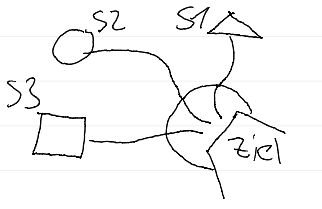
\includegraphics[width=1\linewidth]{content/pictures/Startplaces_Sketch.png}
\caption{Sketchzeichnung der Starträume (Quelle: eigene Darstellung)}
\label{fig:sketch-starterrooms}
\end{figure}

Der Watcher muss auch erkennen können, wohin sie gemeinsam gehen müssen. Daher muss die Spielwelt immer so eindeutig sein, dass es entweder ein oder mehrere eindeutige Ziele geben muss, wohin der Player gelotst werden muss. Für einen ersten Abschnitt ist es allerdings einfacher, wenn ein Ziel festgelegt wird, wohin alle Wege führen. In Abbildung \ref{fig:sketch-starterrooms} ist dieses klar im Sketch zu sehen. 

Die mit der Spielmechaniken einhergehenden Grundmechaniken und Aufgaben des Watchers müssen ebenfalls erlernt werden, darunter zählen das Platzieren, Previewen und Entfernen von Gegenständen. Das Platzieren von Gegenständen kann so initialisiert werden, dass der Watcher zum Start des Spiels bereits einen Gegenstand wie eine Säule im Inventar hat, welche nun nur noch den Ort benötigt, wo sie platziert werden kann. Durch ein weiteres Hindernis und dem Erkennen, dass der Player einen Gegenstand benötigt den er in eine bestimmte Stelle platzieren muss, bekommt der Watcher die Aufforderung dem Player einen bereits existierenden Gegenstand (bspw. eine Fackel) zu schicken. Das Entfernen von Gegenständen kann so so initialisiert werden, dass der Player in der in der Sketchzeichnung eingezeichneten Ziel-Eingangshalle ist (vgl. Abbildung \ref{fig:sketch-starterrooms}) und dort eine Tür oder ähnliches zu einem weiteren Abschnitt öffnen muss. Es werden allerdings wieder die gleichen Gegenstände benötigt, die sie in den vorangegangenen Rätseln verwendet haben. Also müssen die in der Welt platzierten Gegenstände entfernt und erneut platziert werden.

% [Einfügen von unterschieden in der Spielwelt, erklärend aus Feedback vom vorangegangenen Projekt und hier eimbauen wie es in der Umsetzung aussehen kann]
Darüber hinaus lernt der Watcher die Spielkarte richtig zu deuten. Es gibt in der Darstellung der Spielwelt in der Player-Anwendung teilweise kleine Unterschiede zu der des Watchers. Dieser Aspekt soll zudem die Kommunikation fördern. Umgesetzt ist dieser Aspekt durch fehlende Türen in den Starträumen, in denen der Player zu Beginn des Spiels ist, oder bei den Durchgängen zum Eingangsportal zum nächsten Abschnitt.

Analog zum Watcher, erhält der Player ebenfalls eine kleine Einweisung in die Steuerungsmechaniken der Anwendung. Im Allgemeinen sind in der Anwendung des Players Rätsel und Hindernisse eingebaut, partiell allerdings in der Anwendung des Watchers. Aus diesem Grund muss der Player Rätsel/ Hindernisse und Hinweise identifizieren und verwenden können. Um einen ersten Anhaltspunkt für den Start zu erhalten, sollte in den jeweiligen Starträumen des Players eine kleine Notiz eingebaut werden, welche einen Hinweis auf die Einführung der Mechaniken des Watchers und das Lösen des ersten Hindernisses gibt.
\begin{figure}[ht]
\centering
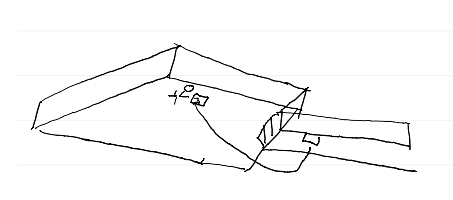
\includegraphics[width=1\linewidth]{content/pictures/Startroom_Sketch.png}
\caption{Sketchzeichnung des Hinweises für das erste Hindernis (Quelle: eigene Darstellung)}
\label{fig:sketch-startriddle}
\end{figure}

Abbildung \ref{fig:sketch-startriddle} zeigt eine erste Überlegung, dass eine Notiz im Startraum darauf aufmerksam macht, dass ein schwerer Gegenstand auf eine Druckplatte gestellt werden muss, durch welche sich die Tür zum anliegenden Flur öffnet.

Außerdem soll der erste Abschnitt das Tragen und Platzieren von Gegenständen enthalten. Es kann also ein Hindernis geben, das über eine Fackelhalterung oder ähnliches gelöst werden kann. Dadurch benötigt der Player einen Gegenstand, den er vom Watcher geschickt bekommt und an die entsprechende Stelle platzieren kann.

Das letzte Lernziel enthält das Freischalten von neuen Abschnitten, das sowohl für den Player als auch den Watcher gilt.

\paragraph{Beschreibung des Abschnittes}

\begin{figure}[ht]
\centering
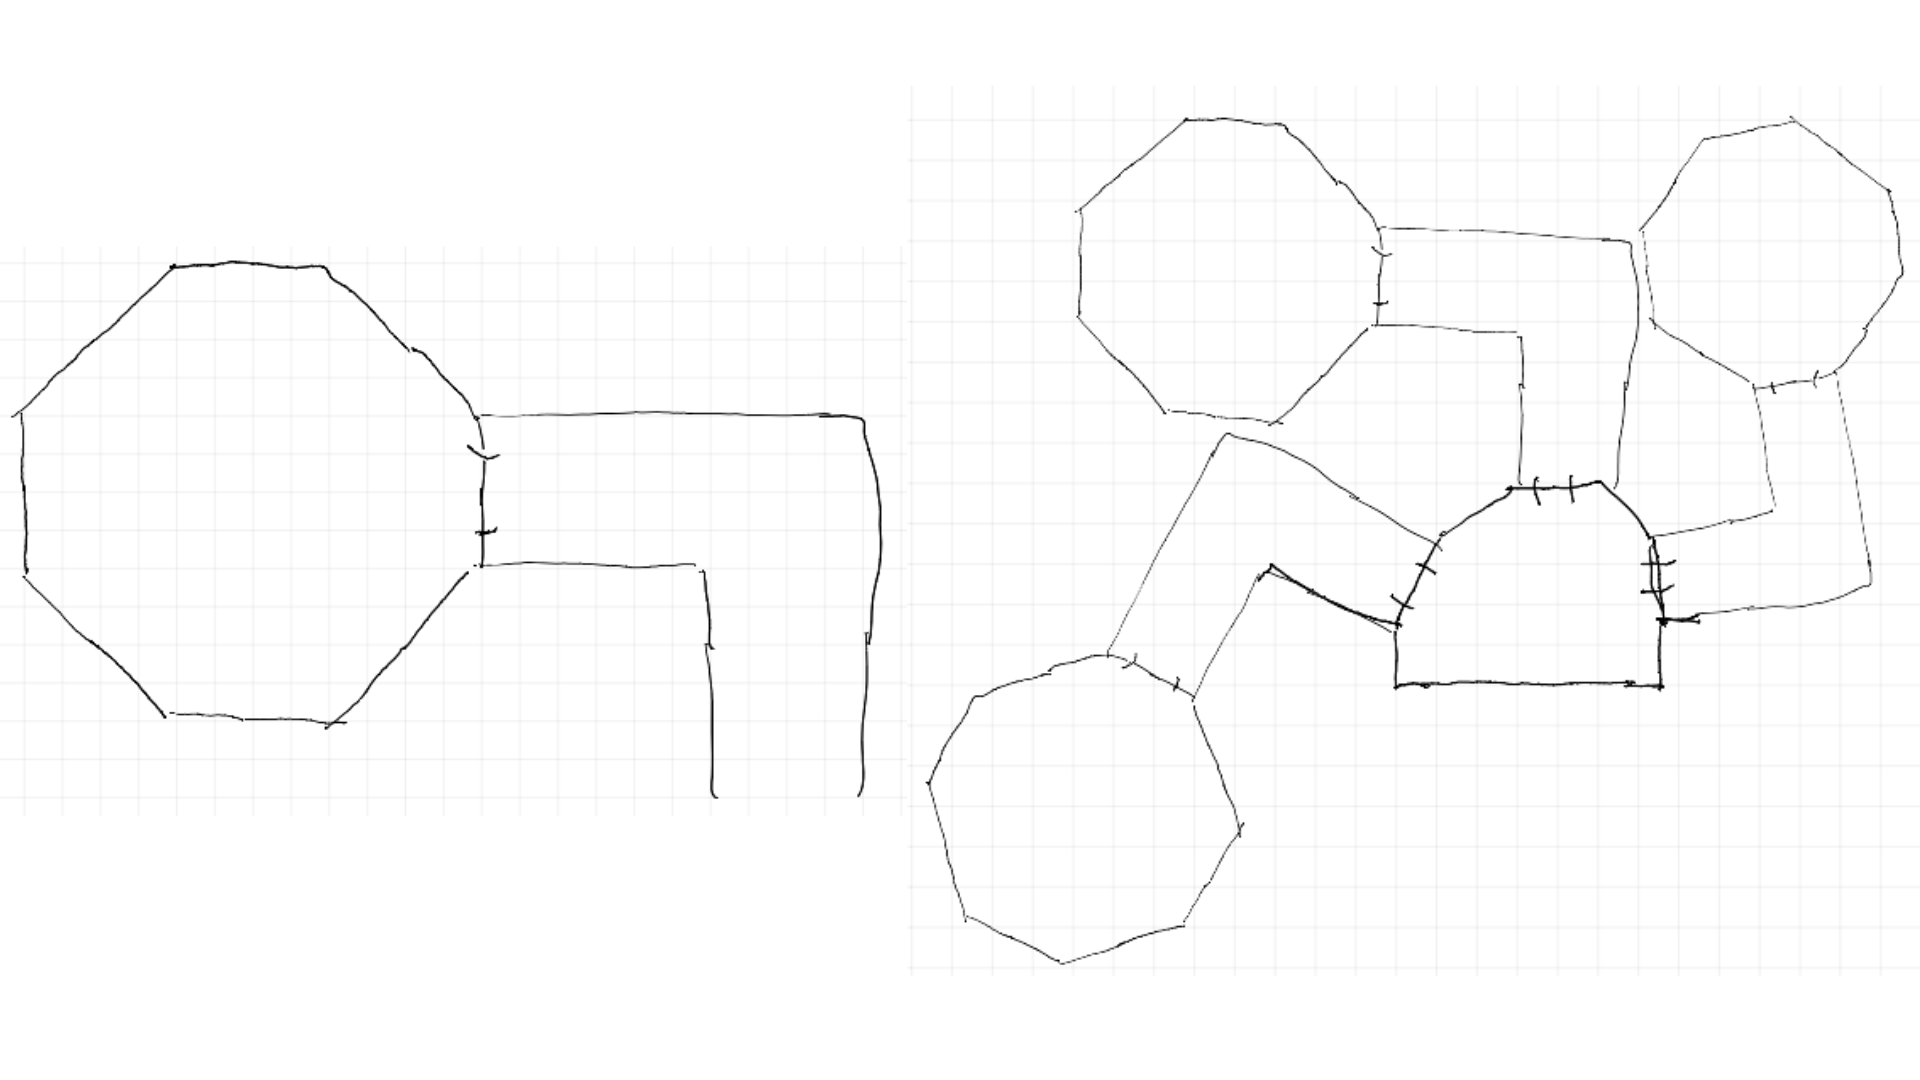
\includegraphics[width=1\linewidth]{content/pictures/Abschnitt_Concept_00.png}
\caption{Konzept Abschnitt 1 (Quelle: eigene Darstellung)}
\label{fig:section_00_concept}
\end{figure}

Abbildung \ref{fig:section_00_concept} zeigt eine erste Konzeptzeichnung des ersten Abschnittes. Sie beinhaltet links einen sechs-eckigen Raum, in dem der Spieler-Avatar des Players in die Spielwelt gesetzt wird. Diesen ersten Startraum gibt es, wie man auf der rechten Seite des Bildes sehen kann drei mal. Der Player muss seinem Watcher nun beschreiben in welchem der drei Räume er sich befindet. Die Räume unterscheiden sich dabei in ihrer Gestaltung. Wie in Abbildung \ref{fig:corridors} zu sehen, besitzt der erste Raum (erste Reihe, linkes Bild) einen Kronleuchter in der Mitte des Raumes, der zweite Raum (zweite Reihe, linkes Bild) einen großen Teppich und der dritte Raum (dritte Reihe, linkes Bild) eine Bank zwischen zwei Innensäulen.

\begin{figure}[ht]
\centering
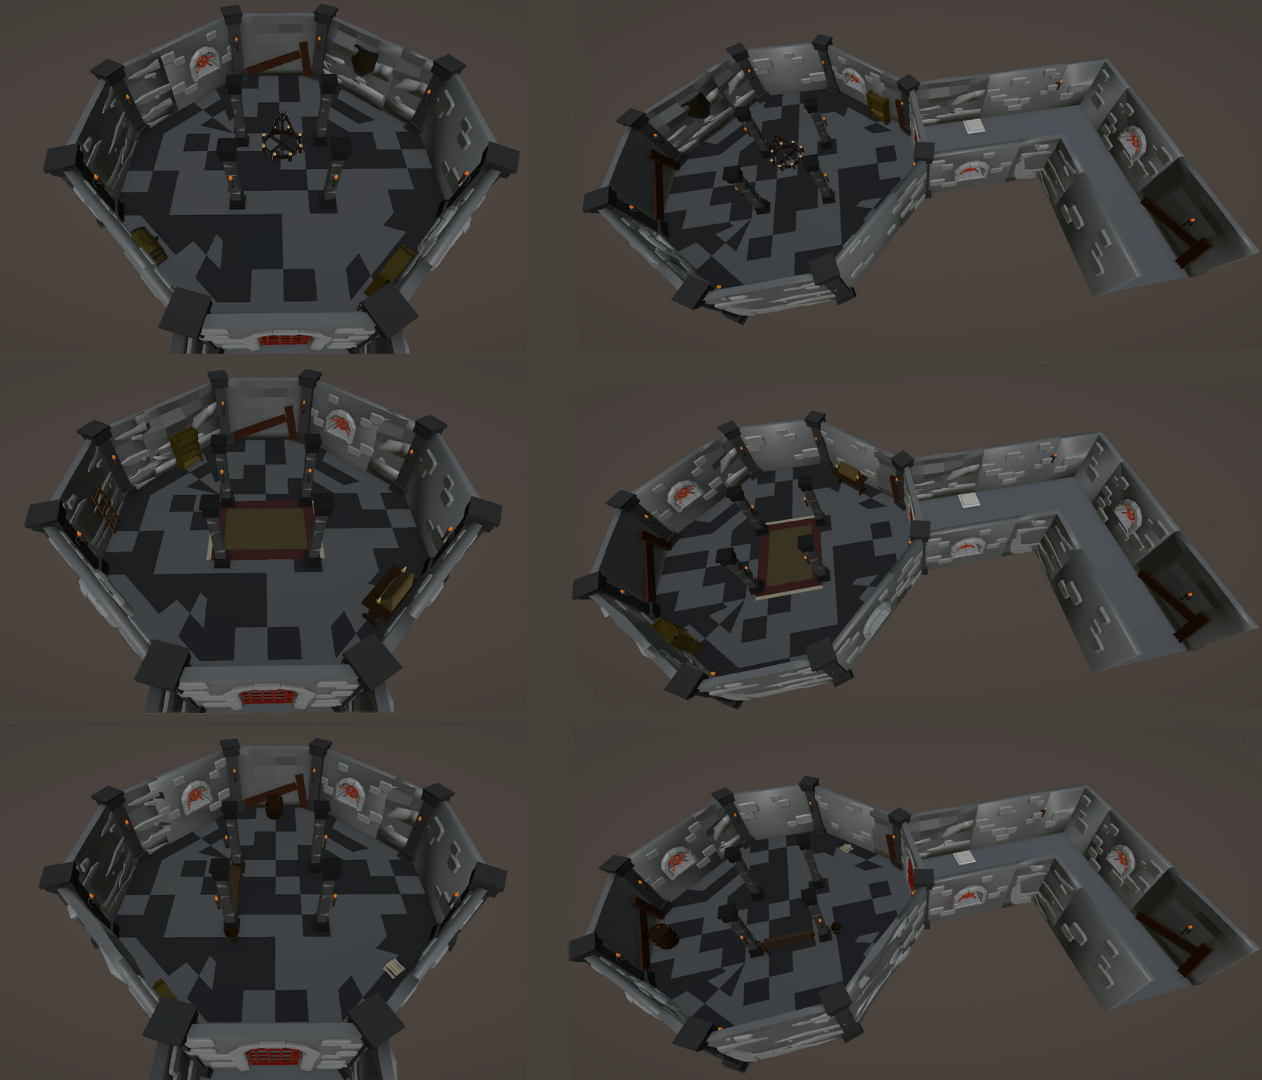
\includegraphics[width=1\linewidth]{content/pictures/Room_00-Room_02-Corridor_00-Corridor_02.png}
\caption{Korridor 1 bis Korridor 3 (Quelle: eigene Darstellung)}
\label{fig:corridors}
\end{figure}

Wie in der Konzeptzeichnung von Abbildung \ref{fig:section_00_concept} im rechten Bild zu sehen, führen die Starträume über einen eckigen Flur in eine Eingangshalle. Dieser ist in Abbildung \ref{fig:section_00} zu sehen. An der entgegenfliegenden Wand von den drei eckigen Fluren aus ist eine Tür, durch die der Player mit Hilfe des Watchers gelangen muss, um den folgenden Abschnitt freizuschalten. 

\begin{figure}[ht]
\centering
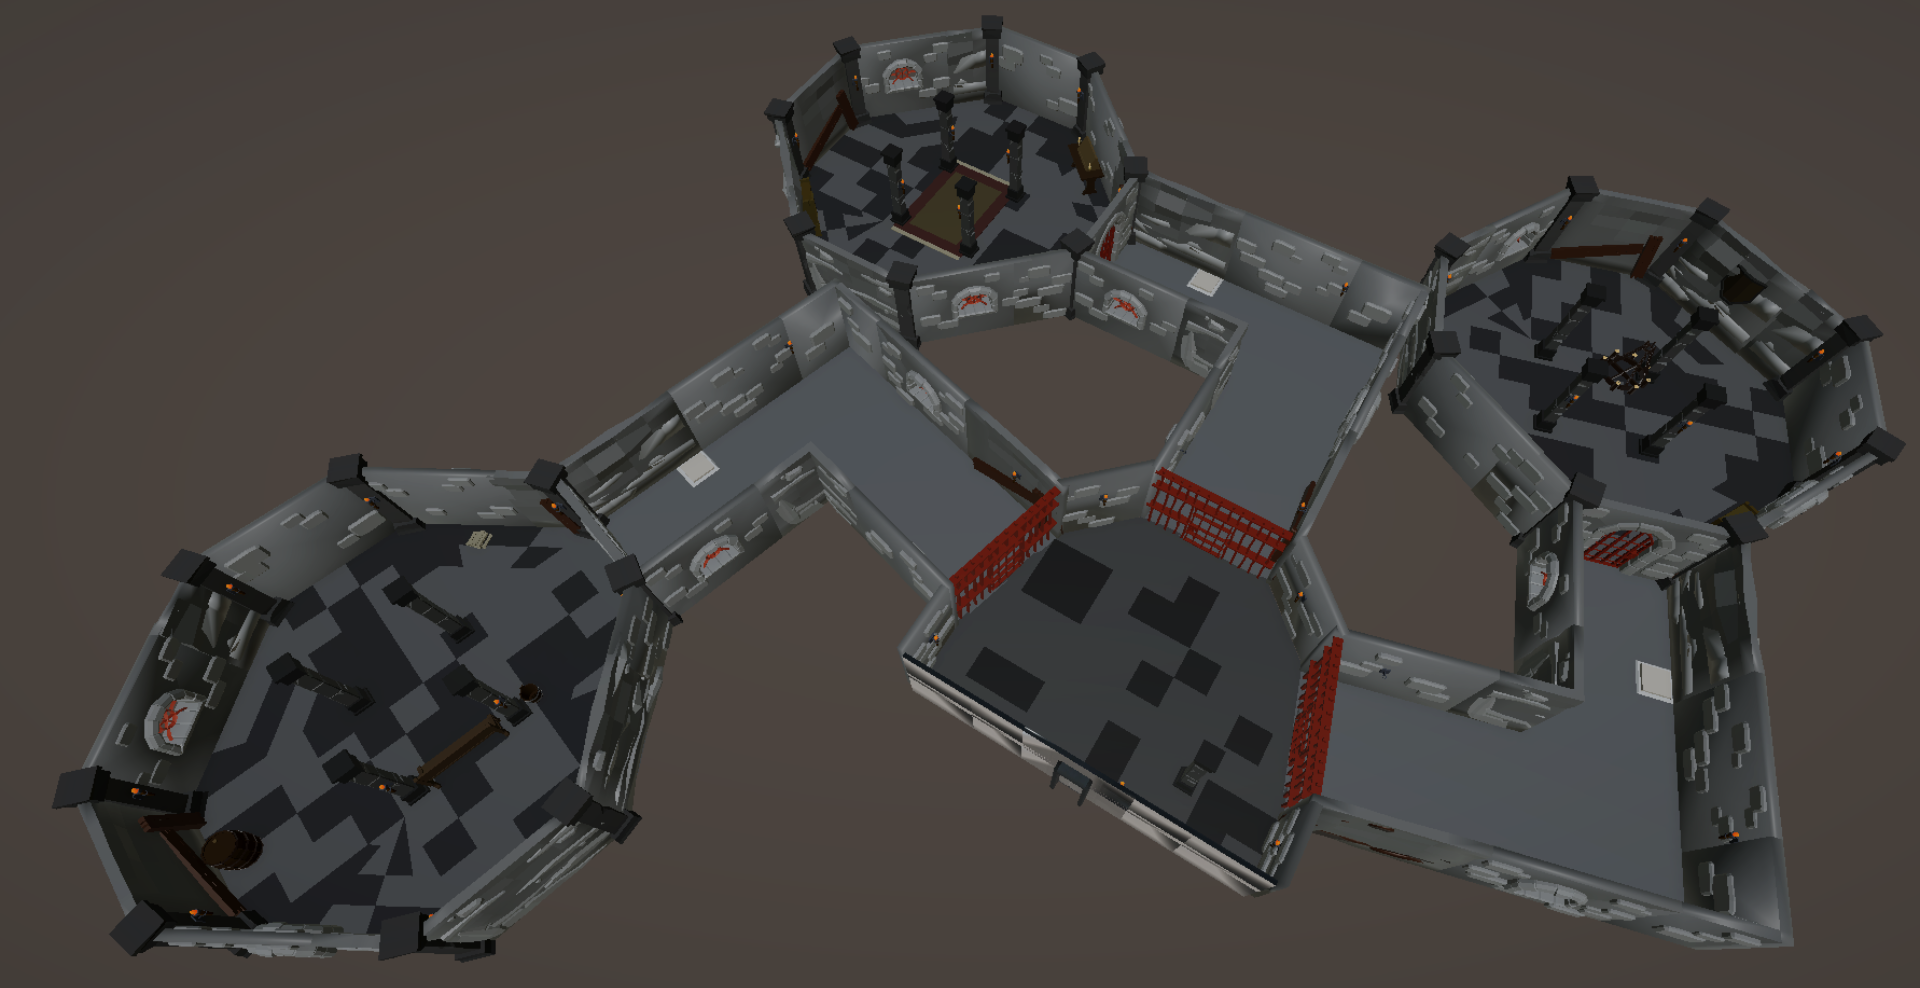
\includegraphics[width=1\linewidth]{content/pictures/Abschnitt_00.PNG}
\caption{Abschnitt 1 (Quelle: eigene Darstellung)}
\label{fig:section_00}
\end{figure}

Der Watcher sieht zum Start den gesamten ersten Abschnitt aus Abbildung \ref{fig:section_00}, wohingegen der Player nur einen der drei Starträume aus Abbildung \ref{fig:corridors} und den anliegenden Flur sehen kann. Die anderen zwei Räume samt Flur kann er nicht sehen. Auch dann nicht, wenn er in die Eingangskammer zum nächsten Abschnitt gelangt ist.

% \paragraph{Lernaspekte dieses Abschnittes}

\subsection{Abschnitt 2: Der Sicherheitsraum}
Analog zu Abschnitt 1 werden zunächst die Lernziele und konzeptionelle Überlegungen vorgestellt. Abschließend wird der Abschnitt vorgestellt.

\paragraph{Lernaspekte und Konzeption dieses Abschnittes}
Im zweiten Abschnitt erlernt der Watcher, dass er weitere Räume sehen kann, die der Player für ihn freigeschaltet hat. Der Player könnte in einem solchen Szenario einen Mechanismus in Gang gesetzt haben, durch welchen ein weiterer Raum für den Watcher sichtbar wurde und in diesem das Rätsel gelöst werden muss.

Außerdem sieht er Gegenstände, welche der Player entdeckt hat als neue platzierte Gegenstände in der Welt und kann diese auch entfernen. Solch ein Gegenstand kann bspw. genutzt werden um ein weiteres Rätsel zu lösen.
In Abhängigkeit davon, erlernt der Player das Entdecken von Gegenständen, durch das nahe an ihnen vorbei gehen. Es kann so umgesetzt werden, dass der Player das Tooltip des Gegenstandes sieht und in diesem Moment der Gegenstand auch für den Watcher sichtbar wird.

\paragraph{Beschreibung des Abschnittes}

\begin{figure}[ht]
\centering
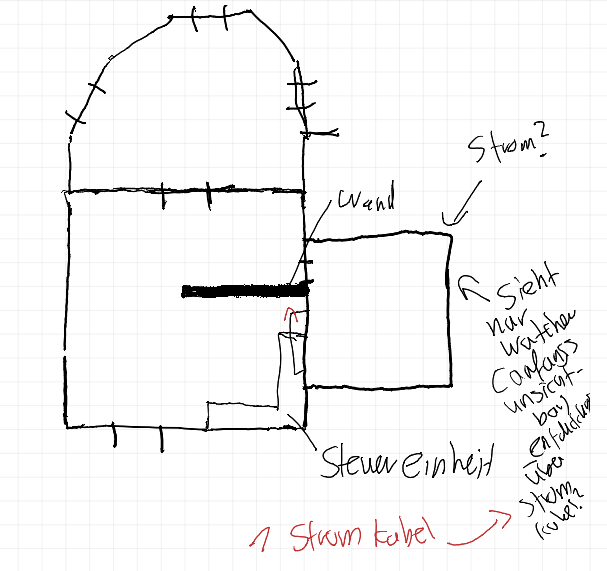
\includegraphics[width=1\linewidth]{content/pictures/Abschnitt_Concept_01.PNG}
\caption{Konzept Abschnitt 2 (Quelle: eigene Darstellung)}
\label{fig:section_01_concept}
\end{figure}

Abbildung \ref{fig:section_01_concept} zeigt eine erste Konzeptzeichnung des zweiten Abschnitts. Gedacht ist dieser als Sicherheitsraum, der ein Verbindungsstück zwischen dem zuvor beschriebenen Verlies ????wo wurde ein Verlies beschreiben???????und den folgenden Räumlichkeiten in Abschnitt 3 ist. Der Player gelangt durch den oberen Eingang von der Eingangshalle in den Sicherheitsraum. Der Sicherheitsraum hat auf der rechten Seite eine Tür in einen Innenhof/ zu einem Außenbereich. Er kann durch die untere Tür in einen weiteren Abschnitt gelangen. Wichtig für einen Sicherheitsraum ist das Überwachungsterminal, welches in der unteren rechten Ecke des Raumes zu finden ist. Damit Arbeiter im Sicherheitsraum abgeschirmt von etwaigen anderen Mitarbeitern oder Personal sind, ist zwischen der Tür auf der rechten Seite und dem Terminal eine Trennwand eingebaut.

\begin{figure}[ht]
\centering
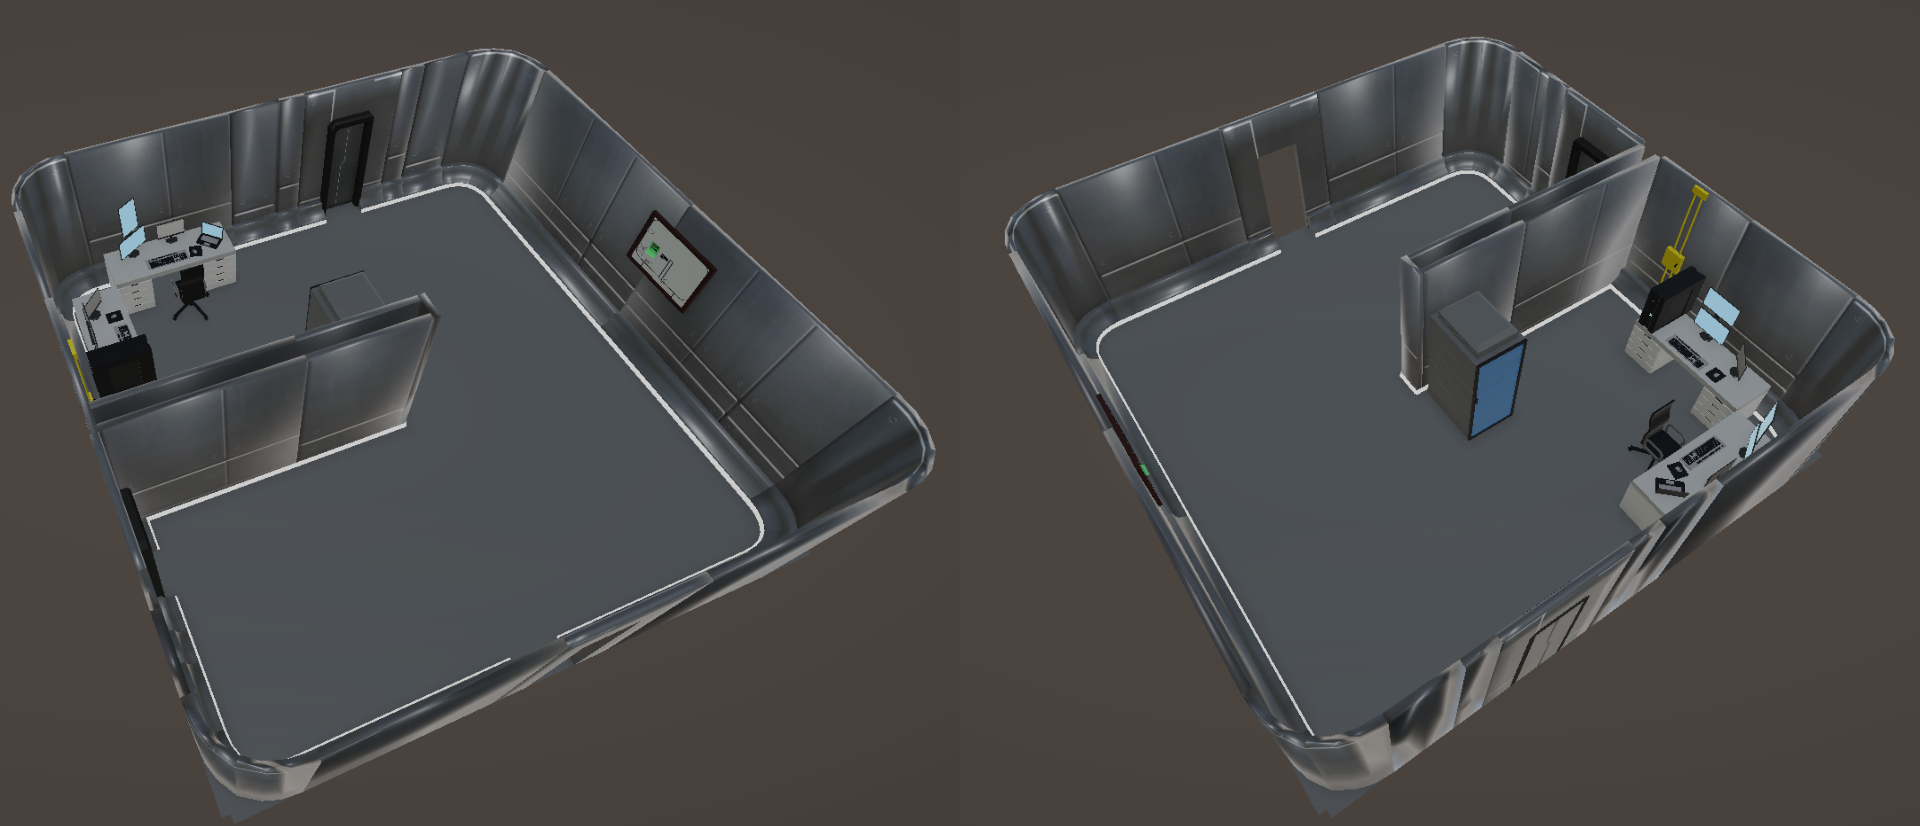
\includegraphics[width=1\linewidth]{content/pictures/Abschnitt_01 - Player.png}
\caption{Abschnitt 2 aus Sicht des Players (Quelle: eigene Darstellung)}
\label{fig:section_01_player}
\end{figure}

\begin{figure}[ht]
\centering
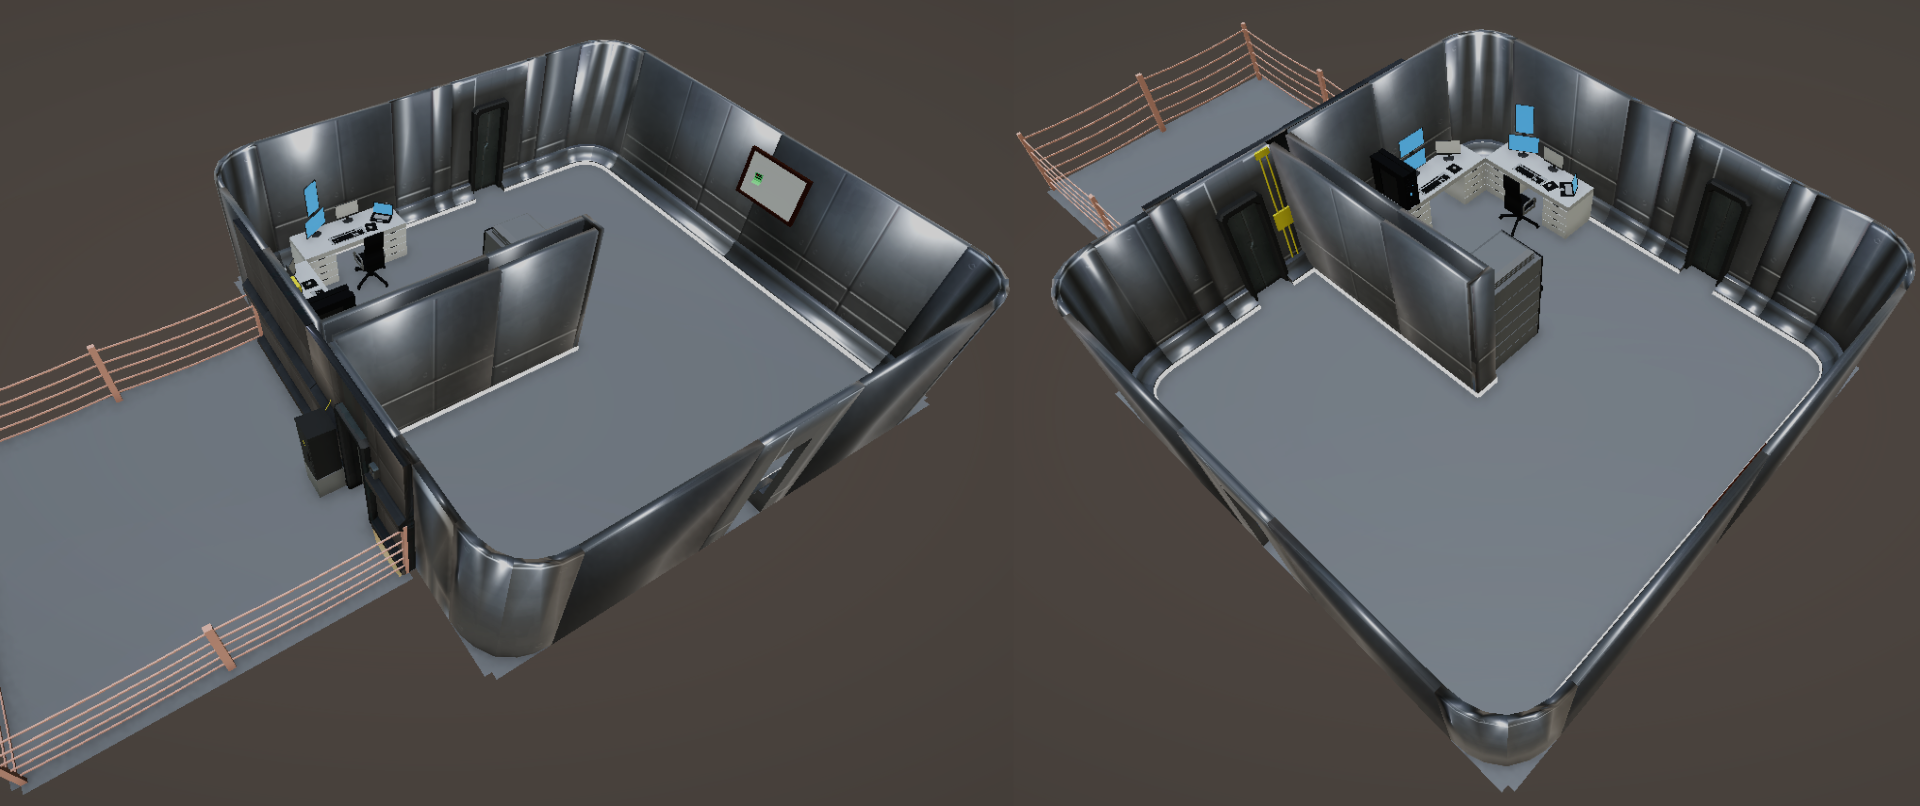
\includegraphics[width=1\linewidth]{content/pictures/Abschnitt_01 - Watcher.png}
\caption{Abschnitt 2 aus Sicht des Watchers (Quelle: eigene Darstellung)}
\label{fig:section_01_watcher}
\end{figure}

Die Abbildungen \ref{fig:section_01_player} und \ref{fig:section_01_watcher} zeigen den Sicherheitsraum in den Varianten der Ansicht von Player und Watcher. Die Unterschiede in den jeweiligen Szenen wurden gezielt so gewählt, dass sich Player und Watcher genauer absprechen müssen wie der Raum bei ihnen aufgebaut ist. Jeder Raum besitzt einen gelben Sicherungskasten mit gelben Leitungen die zu diesem Sicherungskasten hin- und wegführen. In Abbildung \ref{fig:section_01_player} steht dieser im rechten Bild links neben dem PC an der Rückwand zum Außenbereich. In der Anwendung des Watchers steht er im rechten Bild rechts neben der Tür zum Außenbereich (vgl. Abbildung \ref{fig:section_01_watcher}). Auf der Rückseite des Sicherungskasten befindet sich ein Stromgenerator, der im rechten Bild von Abbildung \ref{fig:section_01_watcher} links neben der Tür im Außenbereich zu sehen ist. Simultan zu dem Stromkasten der Player Anwendung fehlt dieser Stromkasten. Das ist für das enthaltene Rätsel wichtig. Wie in den beiden Abbildungen zu sehen ist, sieht nur die Anwendung des Watchers diesen Außenbereich mit dem Stromgenerator. Hier muss der Watcher selbständig durch die Hilfe des Players das enthaltene Rätsel lösen.

\subsection{Abschnitt 3: Das Büro}
Der dritte Abschnitt dient im Tutorial nicht mehr als Lernabschnitt sondern soll direkt als Anwendungsgebiet der erlernten Mechaniken dienen.
Als Szenario wurde hierbei ein Büroabschnitt innerhalb eines größeren Bürokomplexes gewählt. Dieser ist ein Teil des Bürokomplexes aus der Haupthandlung des Spiels. Der vorangegangene Abschnitt diente als Kontrollraum zwischen dem Verlies und dem Bürokomplex.

\begin{figure}[ht]
\centering
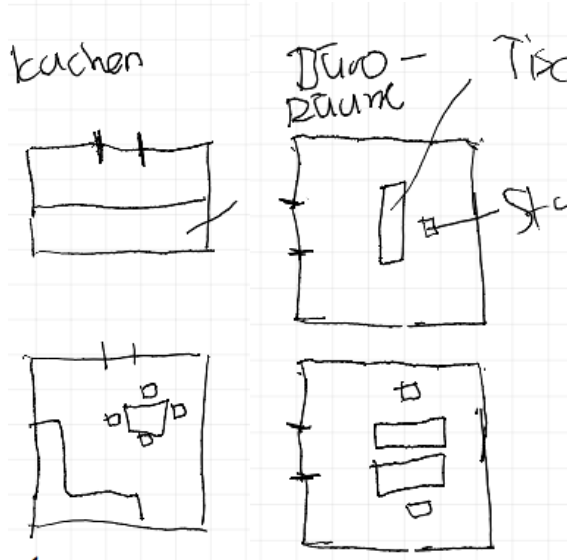
\includegraphics[width=1\linewidth]{content/pictures/Abschnitt_02_Concept.png}
\caption{Konzept Abschnitt 3 (Quelle: eigene Darstellung)}
\label{fig:section_02_concept}
\end{figure}

Abbildung \ref{fig:section_02_concept} zeigt erste Überlegungen für Räume innerhalb des Bürokomplexes. Diese ersten Überlegungen wurden in Abbildung \ref{fig:section_02} erweitert.

\begin{figure}[ht]
\centering
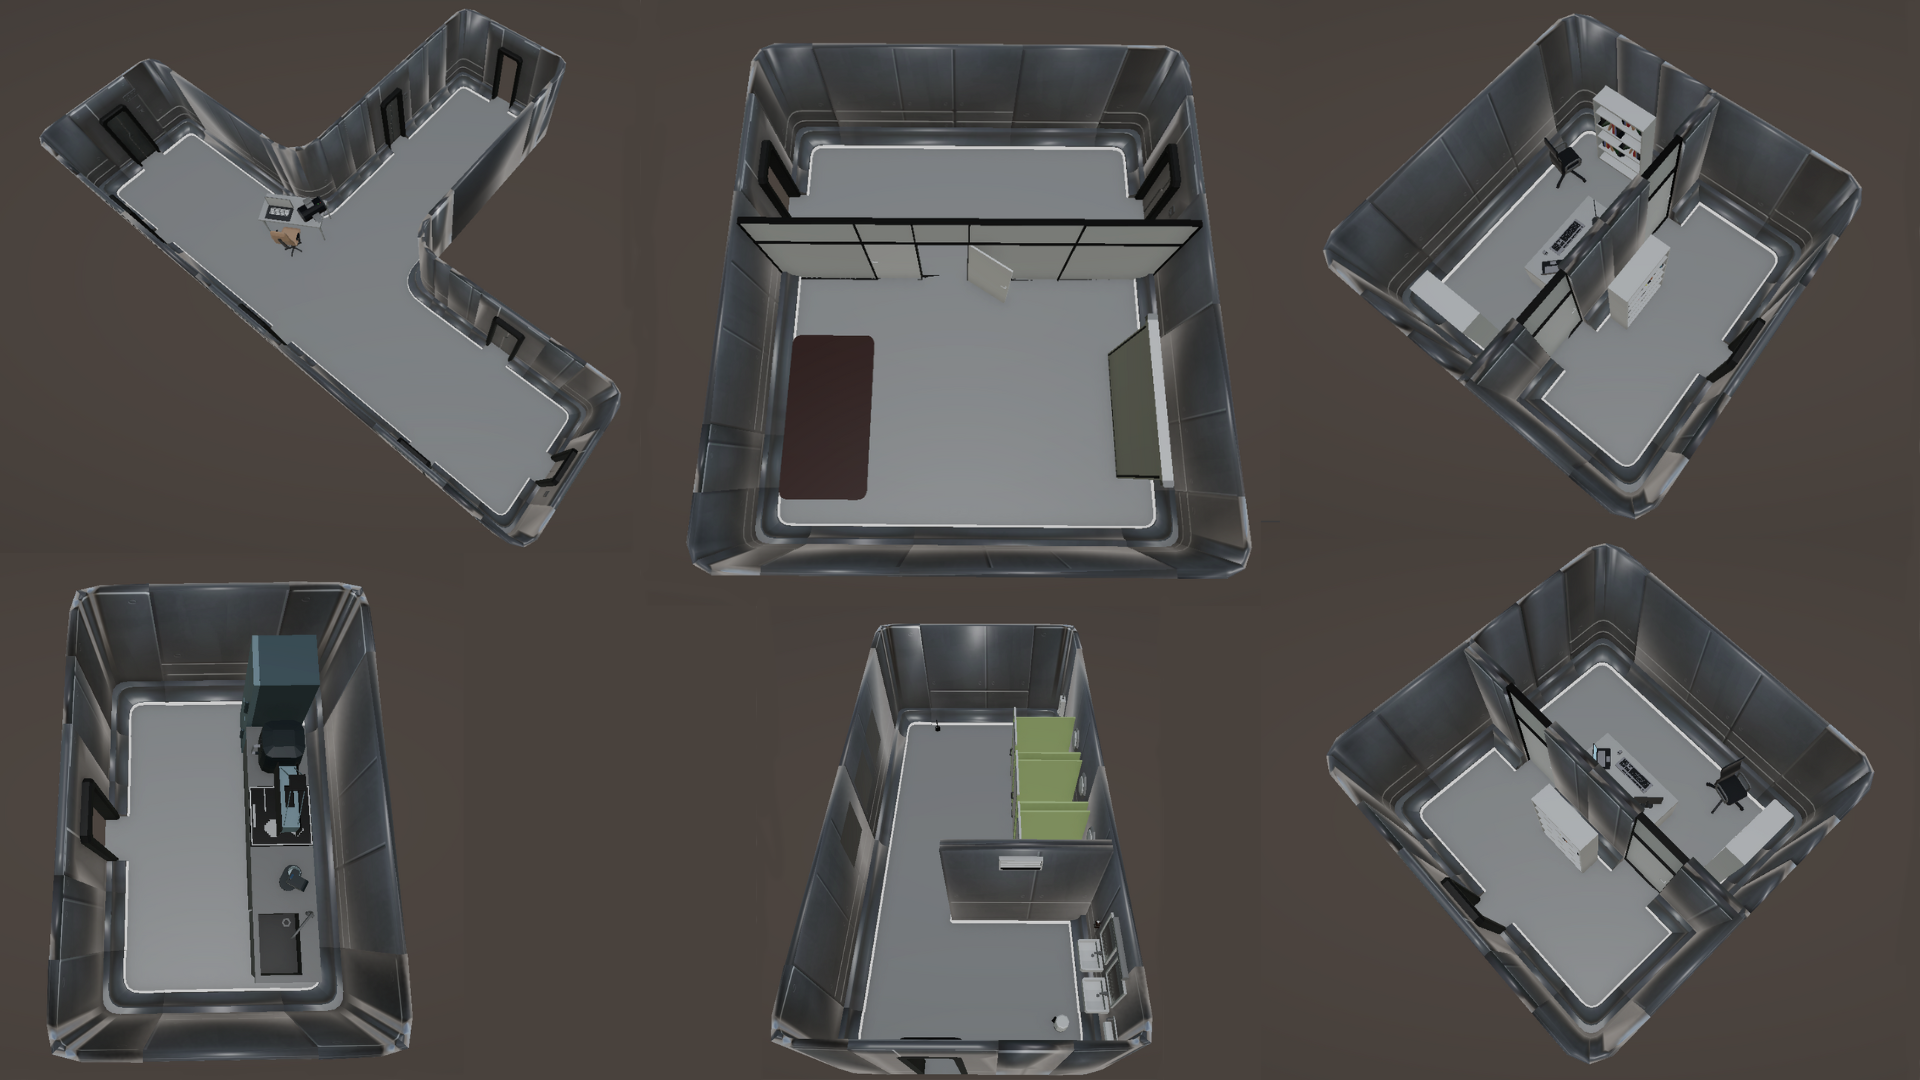
\includegraphics[width=1\linewidth]{content/pictures/Abschnitt_02.png}
\caption{Abschnitt 3 (Quelle: eigene Darstellung)}
\label{fig:section_02}
\end{figure}

Der Bürokomplex im letzten Teil des Tutorials besteht aus einem Korridor (Bild oben links), einer Küche (unten links), einem Tagungsraum (oben Mitte), einem kleinen WC (unten Mitte) und zwei Büros (oben und unten rechts). Auch hier existieren Unterschiede zwischen den Anwendungen des Players und des Watchers. Sowohl der Player als auch der Watcher sehen nur eines der beiden Büros. Sie sind zueinander gespiegelt und enthalten auch ein Rätsel und Hinweise darauf, wie nach Abschließen des enthaltenen Rätsel weiterzumachen ist. In der Anwendung des Players befinden sich im Tagungsraum Stühle, die vom Player entdeckt werden müssen, damit diese für den Watcher von Nutzen sein können. Wie die jeweiligen Räume zusammengehören und welchen Beitrag sie leisten wird im folgenden Kapitel \emph{\nameref{sec:riddles}} erklärt.

\subsection{Rätseldesign}\label{sec:riddles}
Der Aufbau der Rätsel in den Abschnitten 1 und 2 ist linear gehalten, da diese als Einführung in die Mechanik gedacht ist. Die Hinweise der Rätsel sind meist in der Nähe der jeweiligen Rätsel in die Umgebung, oder als Notiz, eingebaut.

\paragraph{Abschnitt 1}

\begin{figure}[ht]
\centering
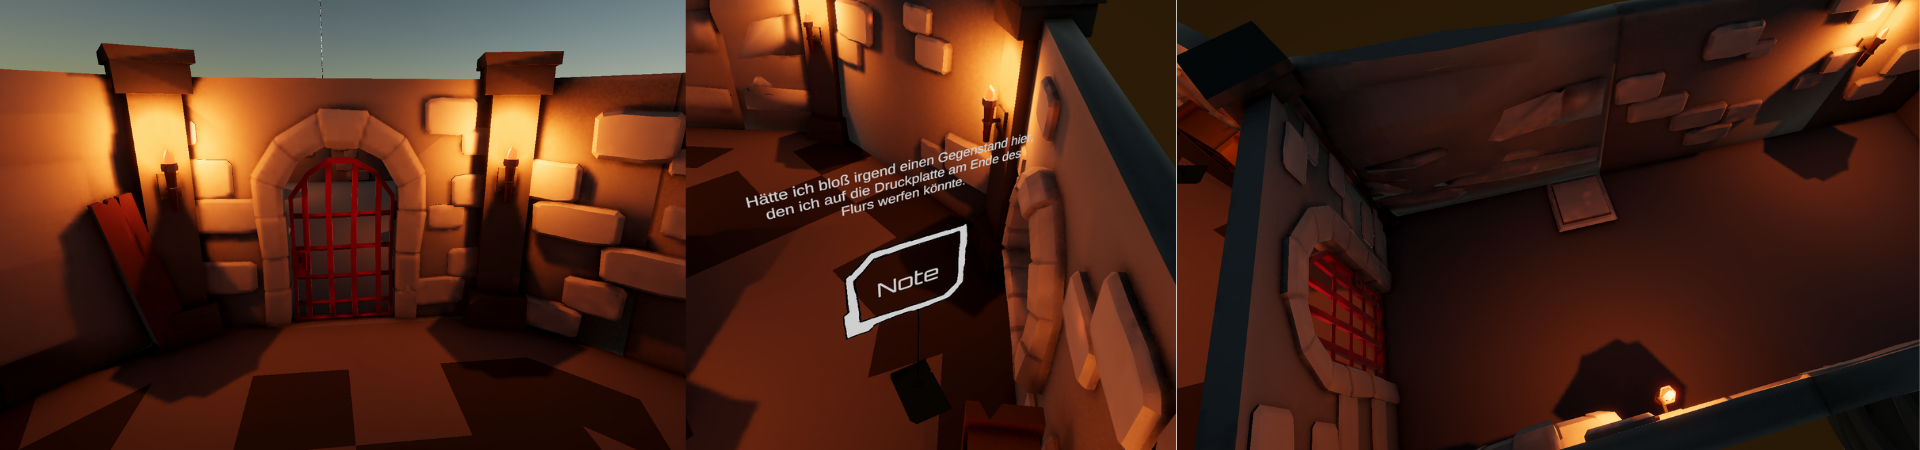
\includegraphics[width=1\linewidth]{content/pictures/Rätseldesign - Abschnitt00 - Rätsel00.png}
\caption{Aufbau der Rätsel von Abschnitt 1, Teil 1 (Quelle: eigene Darstellung)}
\label{fig:riddle-design-section00-00}
\end{figure}

\begin{figure}[ht]
\centering
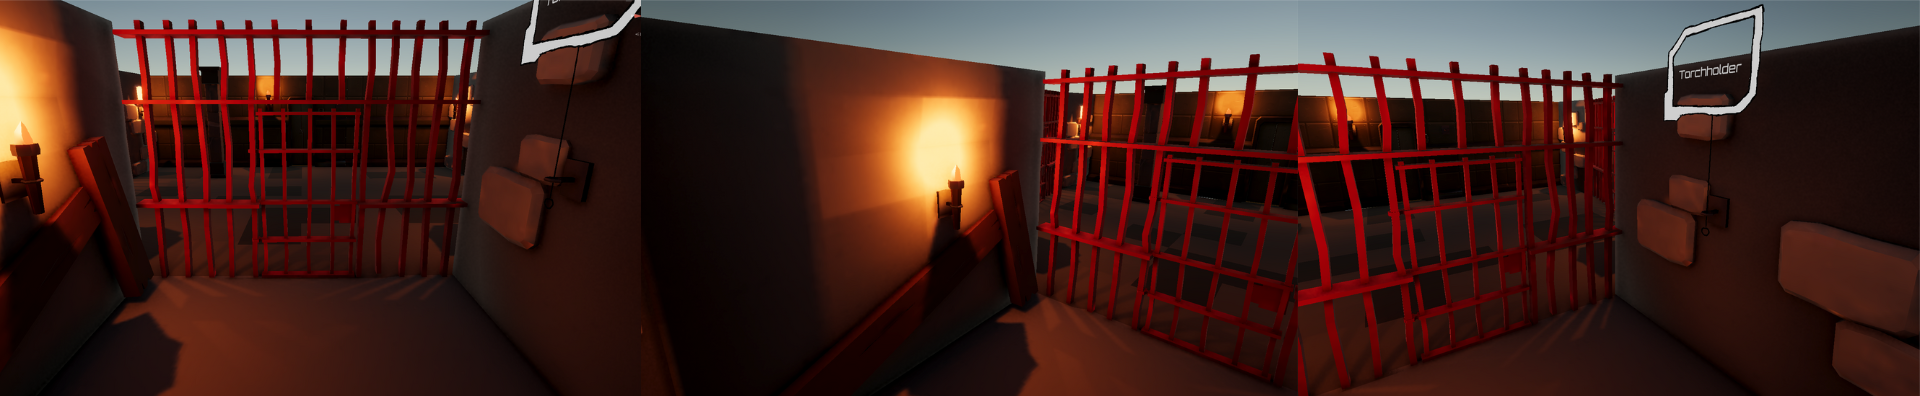
\includegraphics[width=1\linewidth]{content/pictures/Rätseldesign - Abschnitt00 - Rätsel01.png}
\caption{Aufbau der Rätsel von Abschnitt 1, Teil 2 (Quelle: eigene Darstellung)}
\label{fig:riddle-design-section00-01}
\end{figure}

\begin{figure}[ht]
\centering
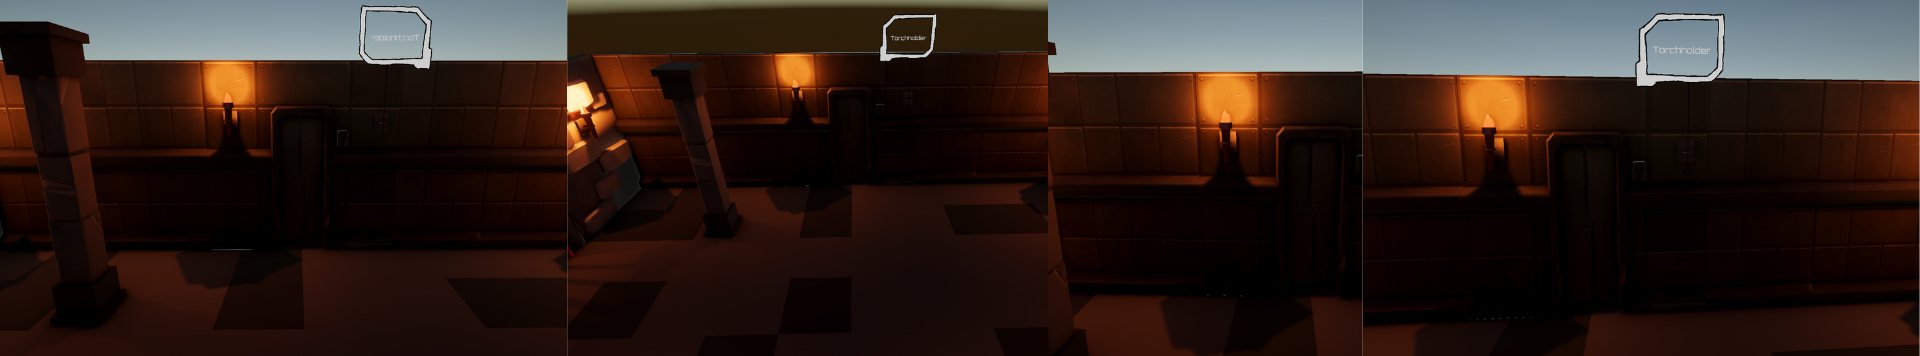
\includegraphics[width=1\linewidth]{content/pictures/Rätseldesign - Abschnitt00 - Rätsel02.png}
\caption{Aufbau der Rätsel von Abschnitt 1, Teil 3 (Quelle: eigene Darstellung)}
\label{fig:riddle-design-section00-02}
\end{figure}

Zum Start befindet sich der Player innerhalb des Verlieses. Eine verrostete Eisentür versperrt ihm den Weg aus dem Verlies (vgl. Abbildung \ref{fig:riddle-design-section00-00}, linkes Bild). Auf einer Notiz (vgl. Abbildung \ref{fig:riddle-design-section00-00}, mittleres Bild) erhält der Player einen Hinweis darauf, auf eine Druckplatte (vgl. Abbildung \ref{fig:riddle-design-section00-00}, rechtes Bild) etwas zu werfen. In diesem Fall ist damit das Platzieren eines schweren Gegenstandes (eine Säule) gemeint, welches zum Start des Spiels im Inventar des Watchers zu finden ist. 

Nachdem der Player aus dem Verlies gelangt ist, stößt er erneut auf eine verrostete Eisentür, welche ebenfalls geöffnet werden muss (vgl. Abbildung \ref{fig:riddle-design-section00-01}, linkes Bild). Auf der von der Tür aus linken Wand, sehen sowohl der Player als auch der Watcher eine Fackelhalterung, in der eine Fackel hängt (vgl. Abbildung \ref{fig:riddle-design-section00-01}, mittlere Bild). Außerdem befindet sich auf der entgegen liegenden Wandseite eine Fackelhalterung ohne Fackel (vgl. Abbildung \ref{fig:riddle-design-section00-01}. rechts Bild). Sie schließen daraus, dass der Watcher dem Player eine Fackel schicken und dieser sie in die Halterung einsetzen muss.

In der folgenden Eingangshalle stoßen beide Spieler auf eine verschlossene Sicherheitstür, welche zum Abschließen des Abschnittes geöffnet werden muss (vgl. Abbildung \ref{fig:riddle-design-section00-02}, linkes Bild). In der Eingangshalle befinden sich links von der Tür eine Säule und eine Fackelhalterung in der eine Fackel steckt (vgl. Abbildung \ref{fig:riddle-design-section00-02}, zweites Bild von links und zweites Bild von rechts). Auf der rechten Seite befindet sich eine leere Fackelhalterung (vgl. Abbildung \ref{fig:riddle-design-section00-02}, rechts Bild). Der Player muss die Fackel, die im vorherigen Rätsel verwendet wurde in die leere Halterung einsetzen. Außerdem muss der Watcher, gemäß der Beschreibung der Säule \say{The column is required to match a pattern or to serve as a counterweight.}, die Säule aus dem ersten Rätsel ungefähr an die auf der rechten Seite der Tür entgegen liegenden Stelle platzieren, sodass die Säulen symmetrisch zur Tür ausgerichtet sind (vgl. Abbildung \ref{fig:riddle-design-section00-02}, linkes Bild).

\paragraph{Abschnitt 2}
In Abschnitt 2 erfolgt das Rätseldesign ähnlich linear wie in Abschnitt 1.

\begin{figure}[ht]
\centering
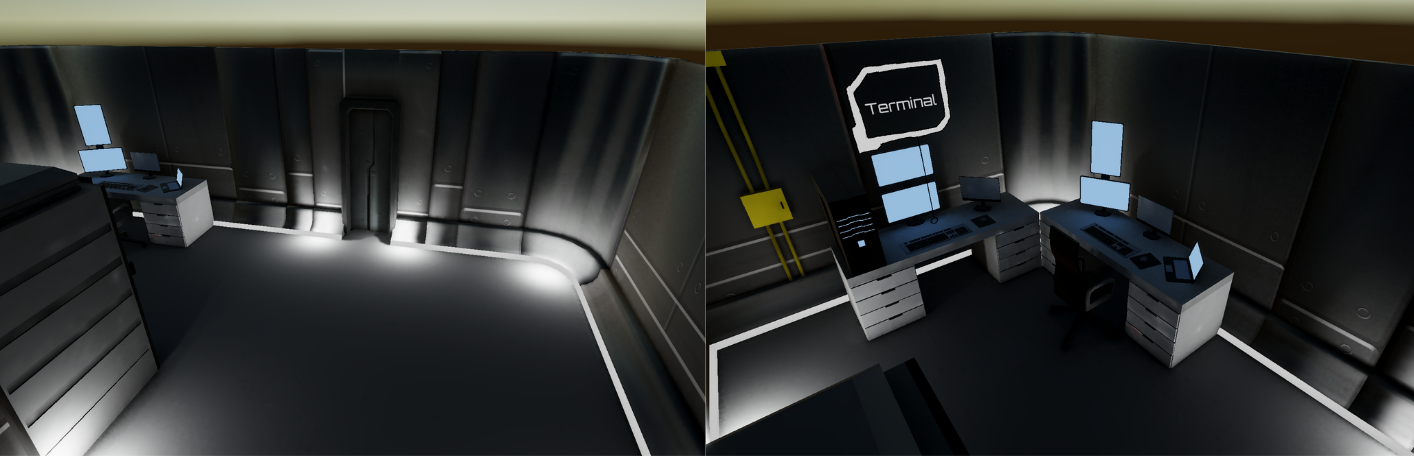
\includegraphics[width=1\linewidth]{content/pictures/Rätseldesign - Abschnitt01 - Rätsel00.png}
\caption{Aufbau der Rätsel von Abschnitt 2, Teil 1 (Quelle: eigene Darstellung)}
\label{fig:riddle-design-section01-00}
\end{figure}

\begin{figure}[ht]
\centering
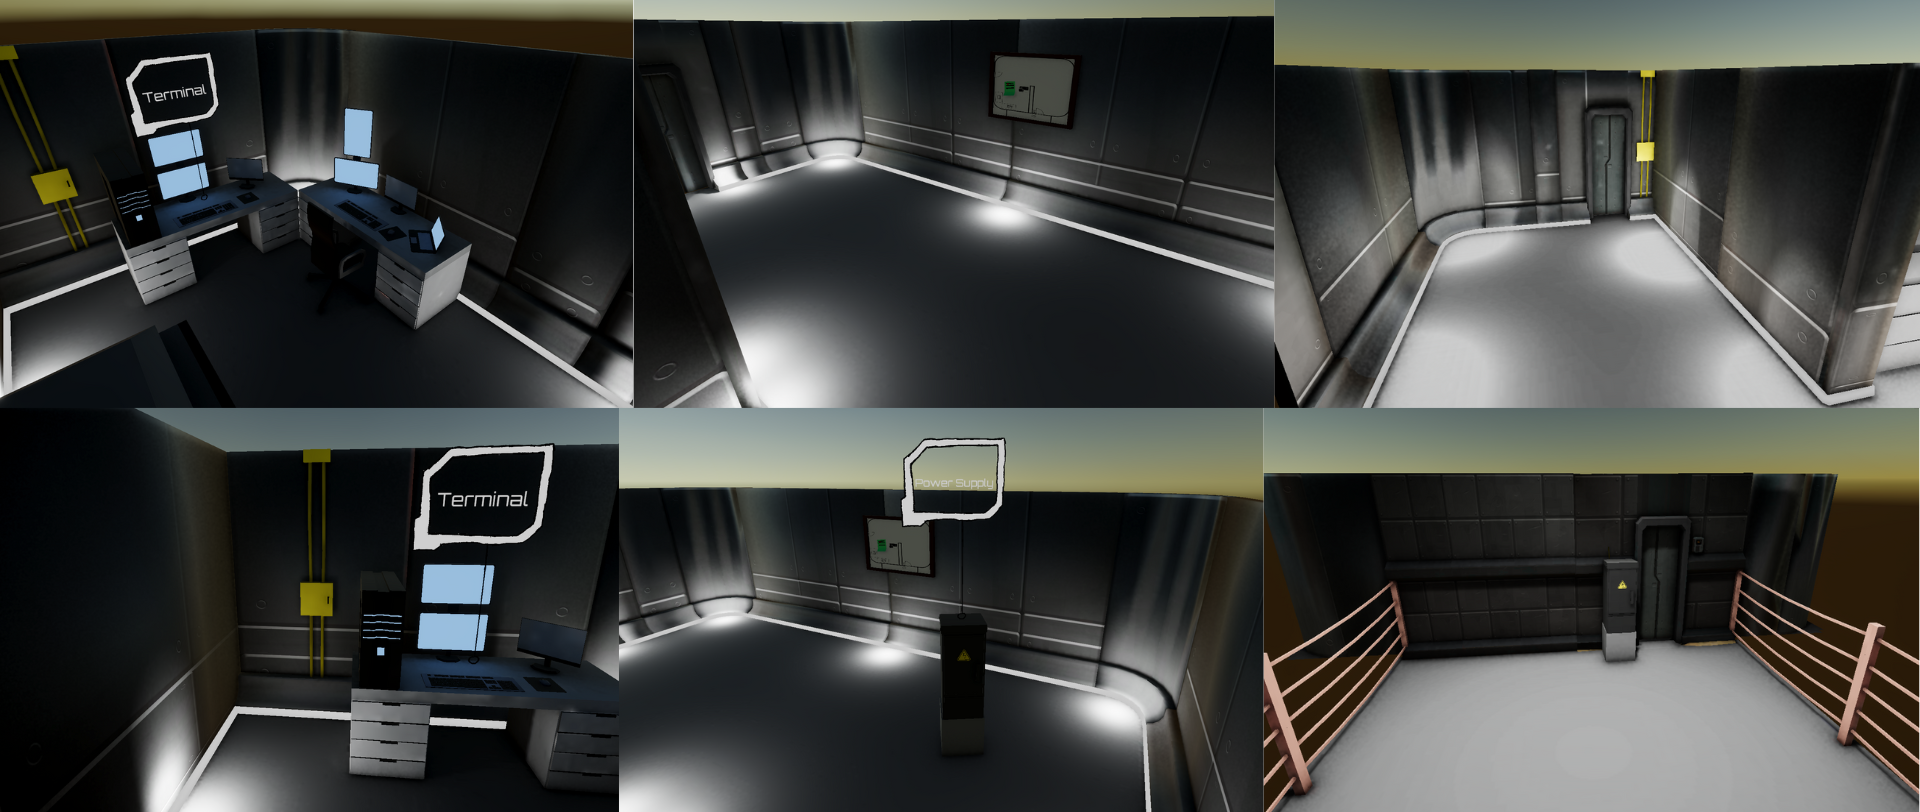
\includegraphics[width=1\linewidth]{content/pictures/Rätseldesign - Abschnitt01 - Rätsel01.png}
\caption{Aufbau der Rätsel von Abschnitt 2, Teil 2 (Quelle: eigene Darstellung)}
\label{fig:riddle-design-section01-01}
\end{figure}

Nachdem der Player in den Sicherheitsraum gegangen ist, stößt er auf 2 Türen. Eine links vom Eingang und eine gegenüber des Eingangs. Durch die gegenüber des Eingangs muss der Player am Ende des Abschnittes gehen. Allerdings geht das zunächst nicht, da der Bewegungsmelder der Tür deaktiviert ist und erst aktiviert werden muss. Am Terminal, das links neben der Tür zu finden ist, muss er Player den Bewegungsmelder aktivieren (vgl. Abbildung \ref{fig:riddle-design-section01-00}). Allerdings besitzt dieses keinen Strom. 

Der Player als auch der Watcher erhalten einige Hinweise darauf, wie der Strom für das Terminal zu aktivieren ist. Zunächst befindet sich innerhalb des Sicherheitsraumes ein Stromgenerator (vgl. Abbildung \ref{fig:riddle-design-section01-01}, Bild zweite Zeile Mitte), welcher an einen anderen Ort platziert werden muss. In der Ansicht des Watchers befindet sich rechts neben der zweiten Tür im Sicherheitsraum, die vom Eingang in den Raum aus links ist, eine Sicherung, auf deren anderen Seite in einem kleinen Innenhof ein Stromgenerator für die Eingangstür steht (vgl. Abbildung \ref{fig:riddle-design-section01-01}, Bilder erste und zweite Zeile rechts). Der Player besitzt für diesen Aufbau, den der Watcher in seiner Version sieht, einen Plan auf einer Pinnwand (vgl. Abbildung \ref{fig:riddle-design-section01-01}, Bild erste Reihe Mitte). Der Unterschied zwischen der Version des Players und des Watchers ist, dass die Sicherung nicht neben der Tür ist, sondern links neben dem Terminal (vgl. Abbildung \ref{fig:riddle-design-section01-01}, Bild zweite reihe links). Aus diesem Grund muss der Generator auf die entgegen liegende Seite links neben den bestehenden Stromkasten in der Anwendung des Watchers (vgl. Abbildung \ref{fig:riddle-design-section01-01}, Bild zweite Reihe rechts) platziert werden. Ist der Generator an dier Stelle platziert, kann der Bewegungsmelder über das Terminal aktiviert werden und der Player kann Abschnitt 3 betreten.

\paragraph{Abschnitt 3}
Abschnitt 3 ist der komplexeste des Tutorials. Player und Watcher erhalten in verschiedenen freigeschalteten Räumen Hinweise oder Gegenstände zu weiteren Rätseln. Die Rätsel werden zu späteren Zeitpunkten benötigt.

\begin{figure}[ht]
\centering
\includegraphics[width=0.7\linewidth]{content/pictures/Rätseldesign_Section02.drawio.png}
\caption{Rätseldesign von Abschnitt 3 (Quelle: eigene Darstellung), vollständig in Anhang: \ref{}}
\label{fig:r
iddle-design-section02-uml}
\end{figure}

Abbildung \ref{fig:riddle-design-section02-uml} zeigt das für das in Abschnitt 3 entworfene Rätseldesign. Dieses Diagramm wird durch die Abbildungen \ref{fig:riddle-design-section02-00} bis \ref{fig:riddle-design-section02-04} vervollständigt.

\begin{figure}[ht]
\centering
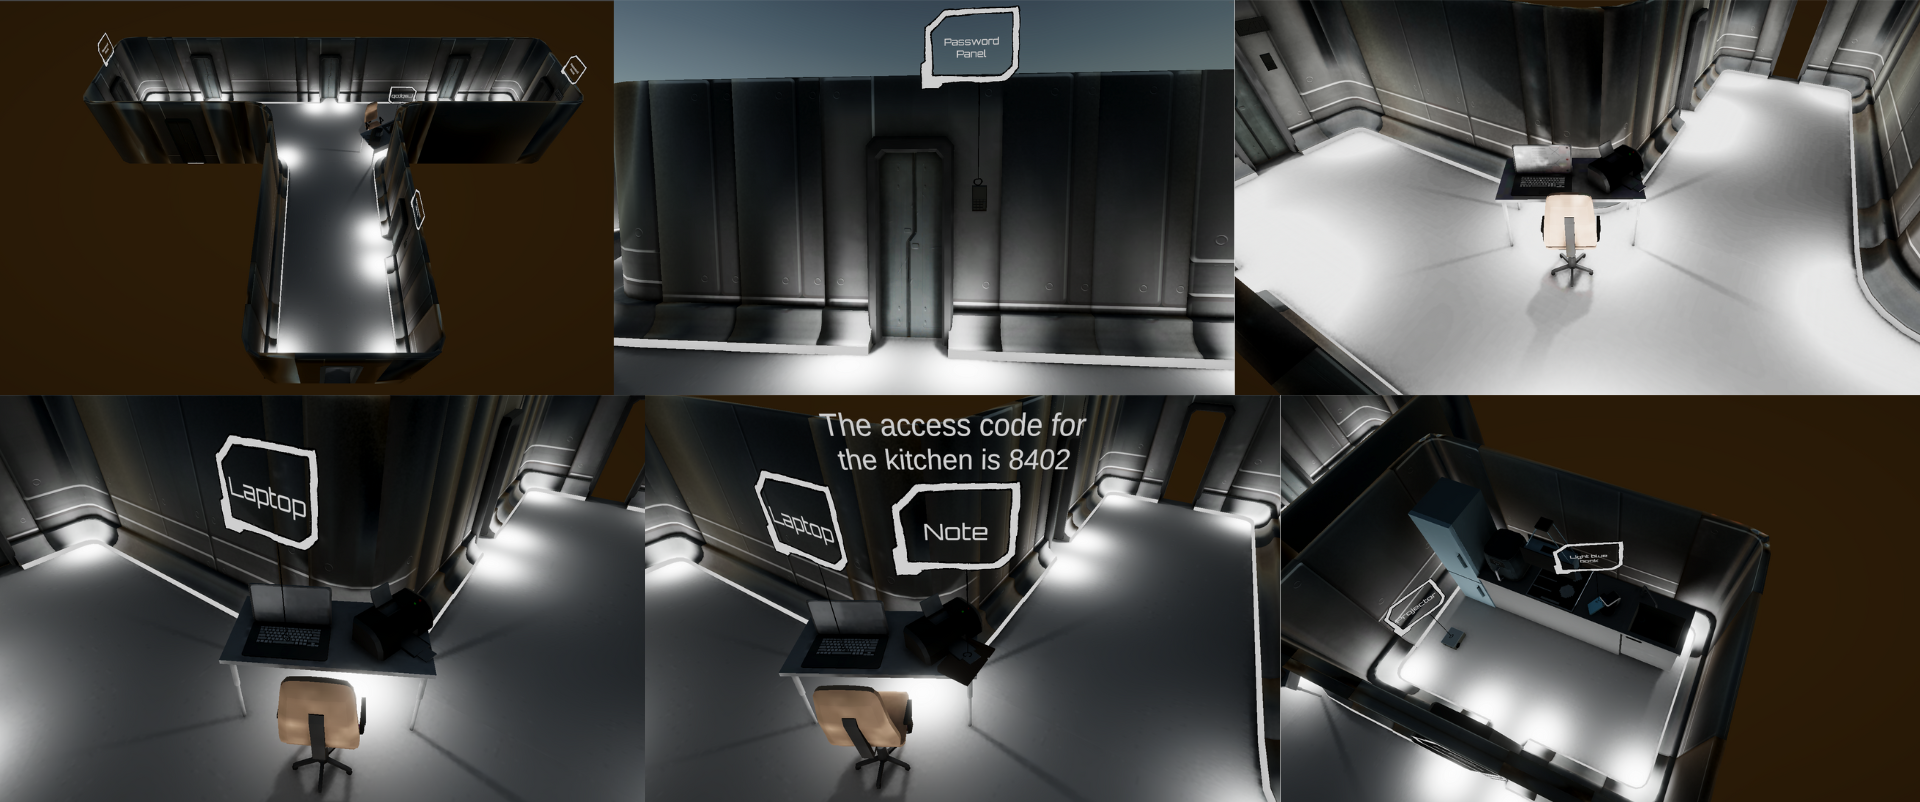
\includegraphics[width=1\linewidth]{content/pictures/Rätseldesign - Abschnitt02 - Rätsel00.png}
\caption{Aufbau der Rätsel von Abschnitt 3, Teil 1 (Quelle: eigene Darstellung)}
\label{fig:riddle-design-section02-00}
\end{figure}

\begin{figure}[ht]
\centering
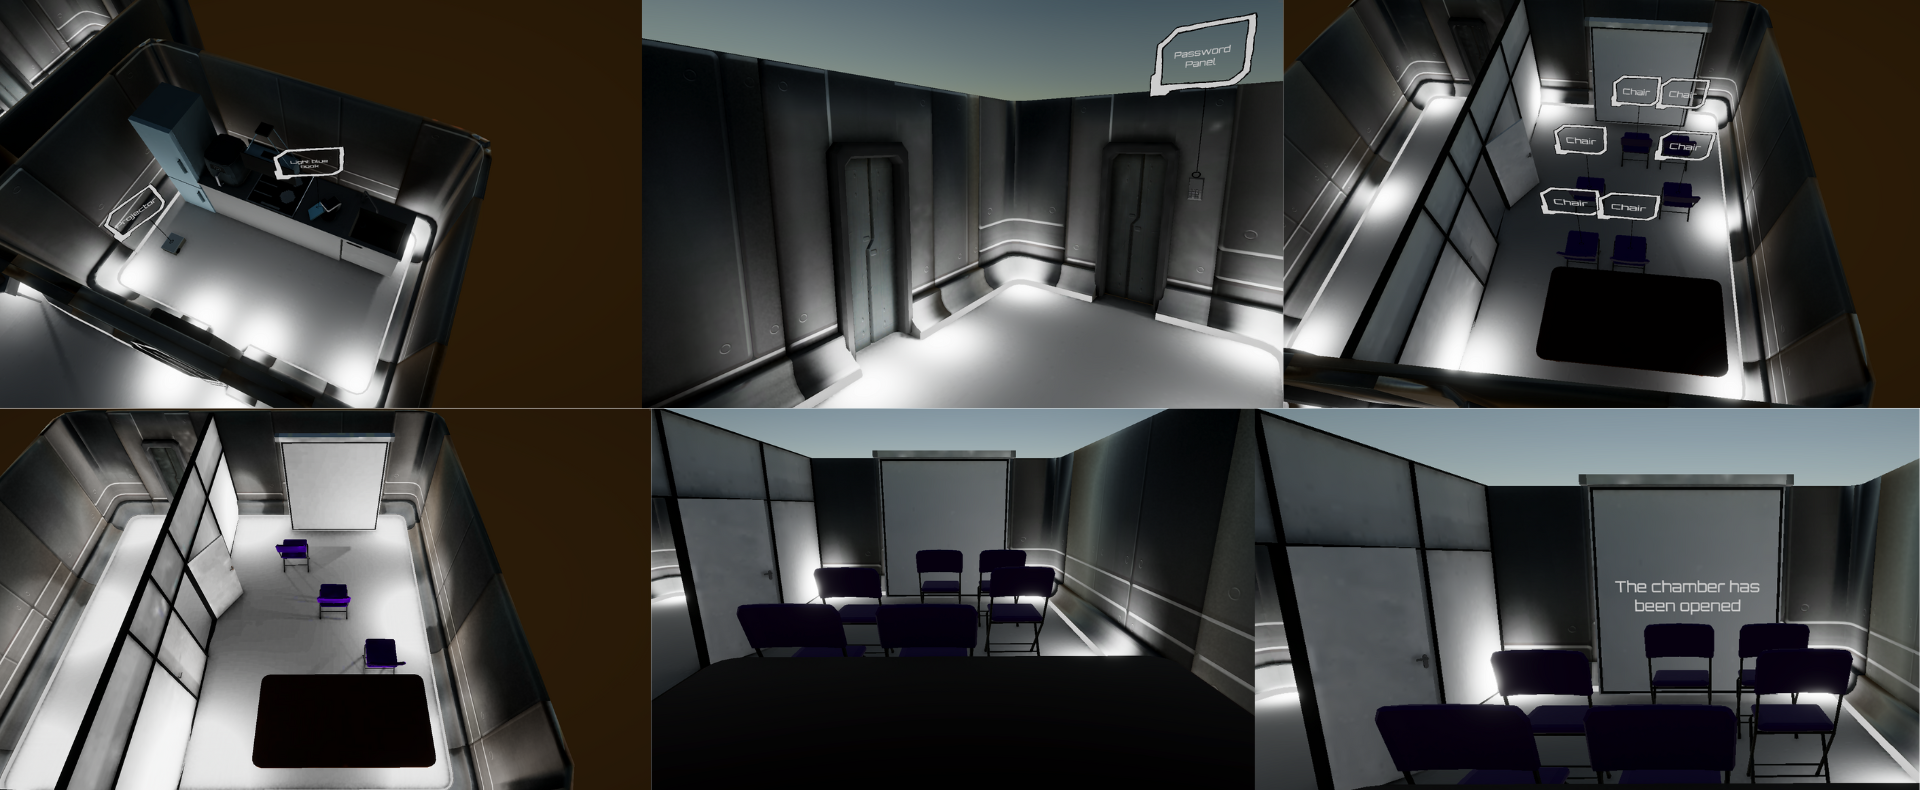
\includegraphics[width=1\linewidth]{content/pictures/Rätseldesign - Abschnitt02 - Rätsel01.png}
\caption{Aufbau der Rätsel von Abschnitt 3, Teil 2 (Quelle: eigene Darstellung)}
\label{fig:riddle-design-section02-0l}
\end{figure}

\begin{figure}[ht]
\centering
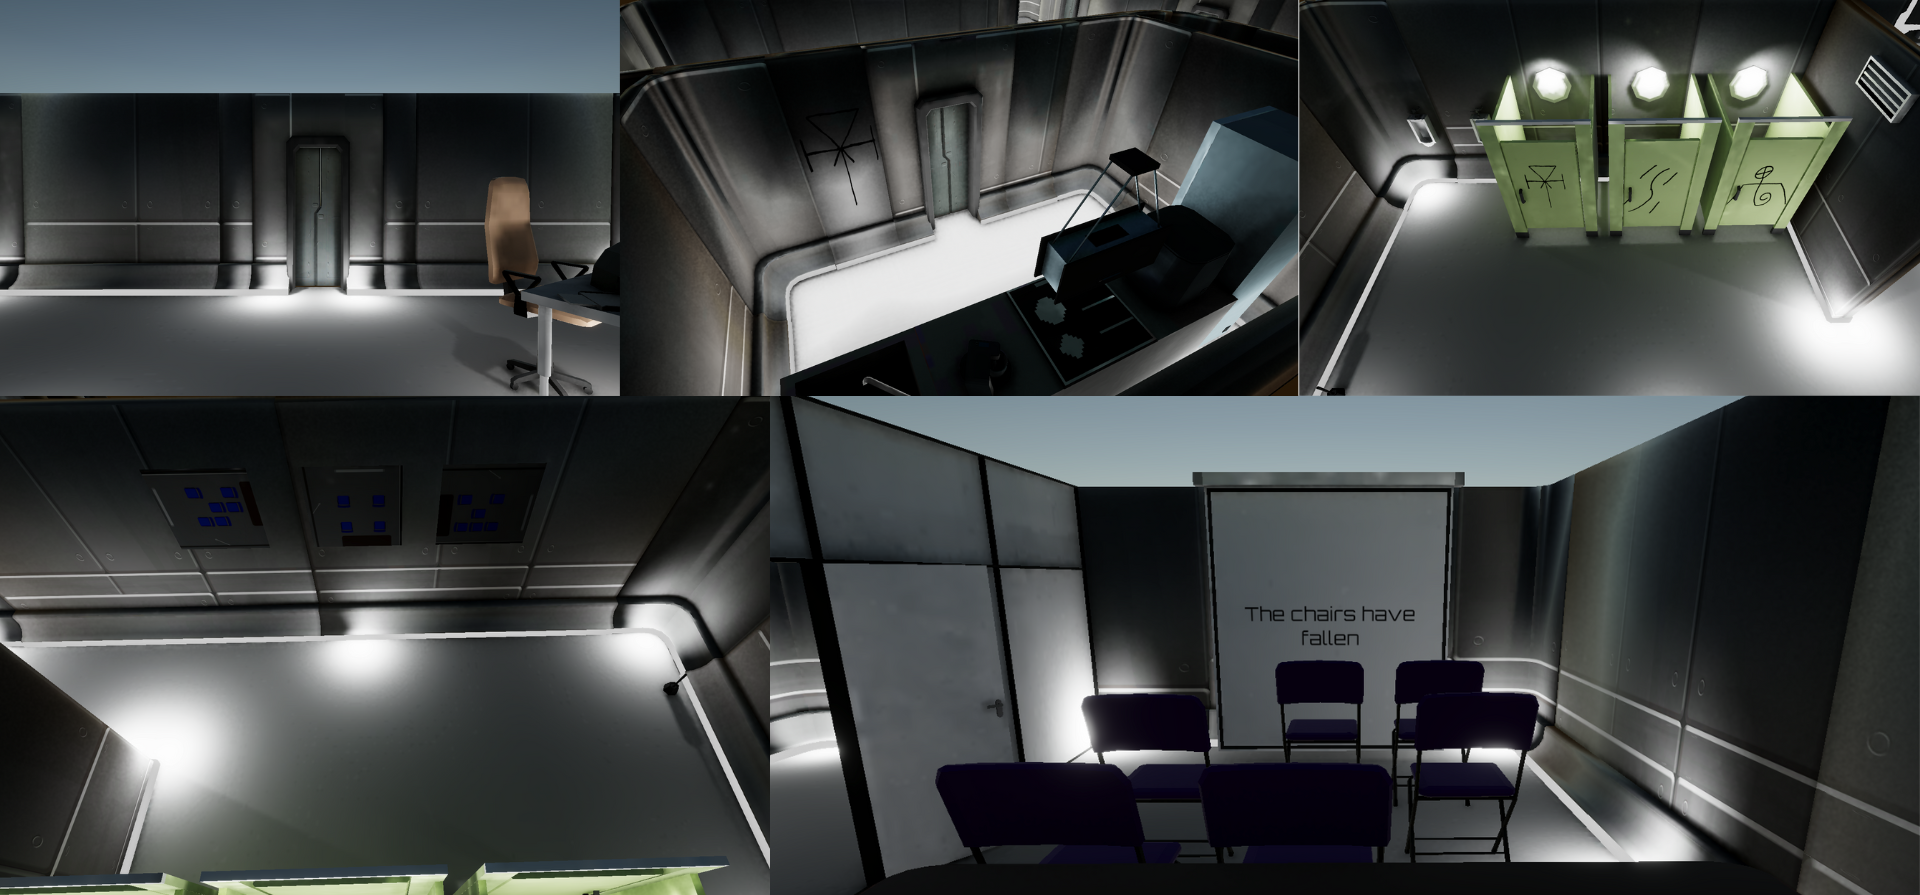
\includegraphics[width=1\linewidth]{content/pictures/Rätseldesign - Abschnitt02 - Rätsel02.png}
\caption{Aufbau der Rätsel von Abschnitt 3, Teil 3 (Quelle: eigene Darstellung)}
\label{fig:riddle-design-section02-02}
\end{figure}

\begin{figure}[ht]
\centering
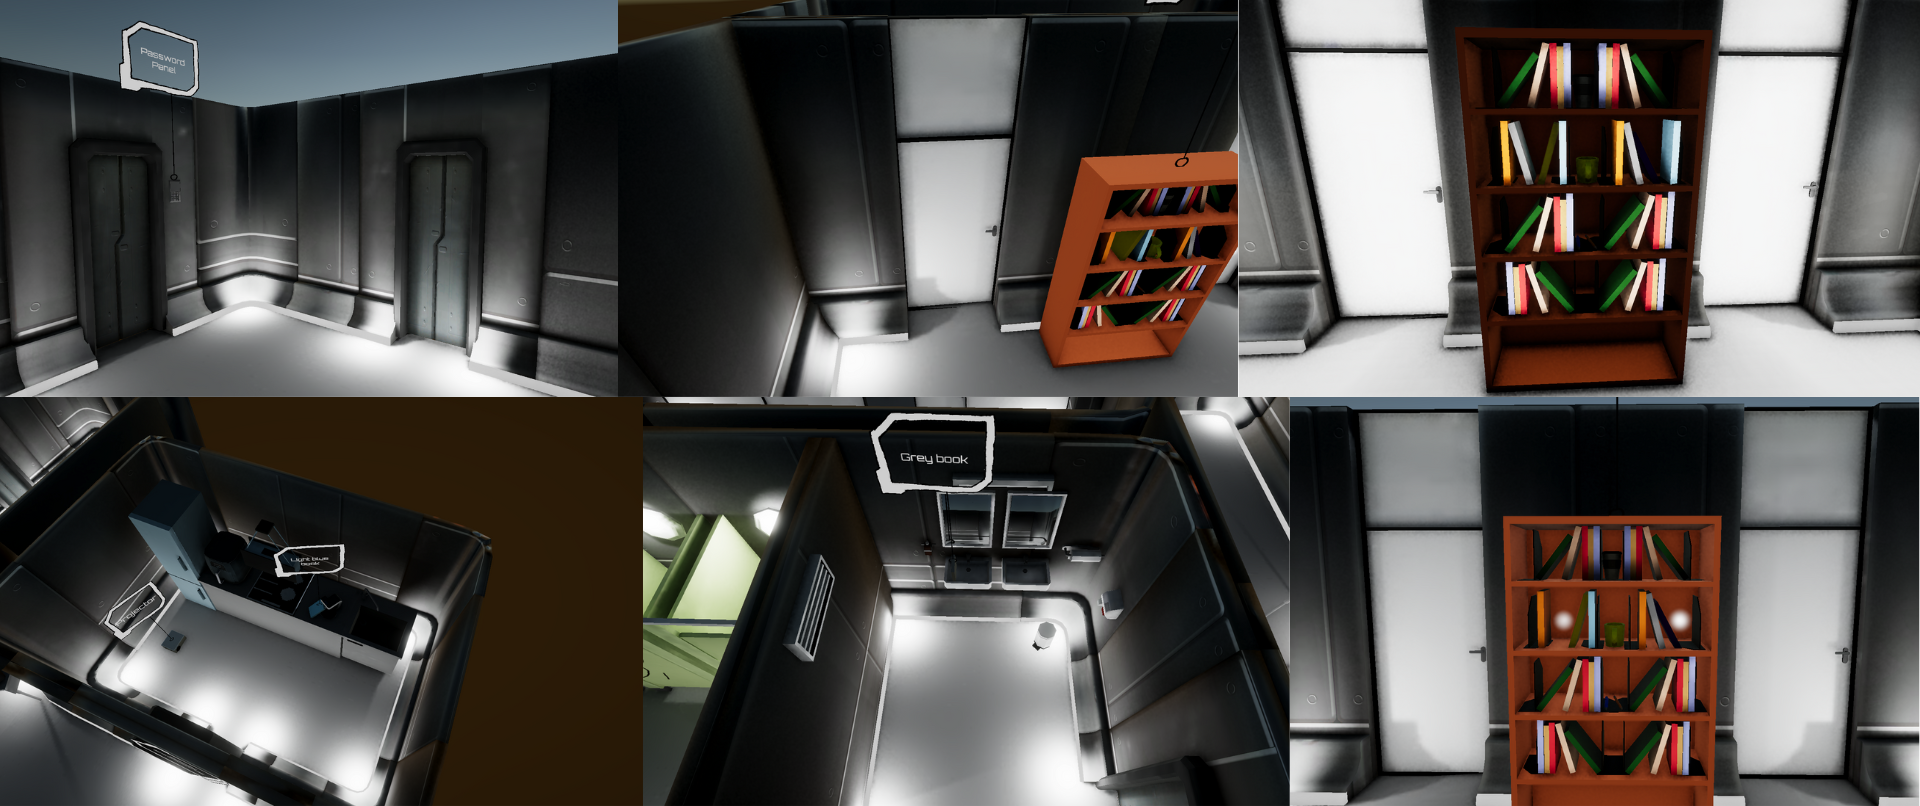
\includegraphics[width=1\linewidth]{content/pictures/Rätseldesign - Abschnitt02 - Rätsel03.png}
\caption{Aufbau der Rätsel von Abschnitt 3, Teil 4 (Quelle: eigene Darstellung)}
\label{fig:riddle-design-section02-03}
\end{figure}

\begin{figure}[ht]
\centering
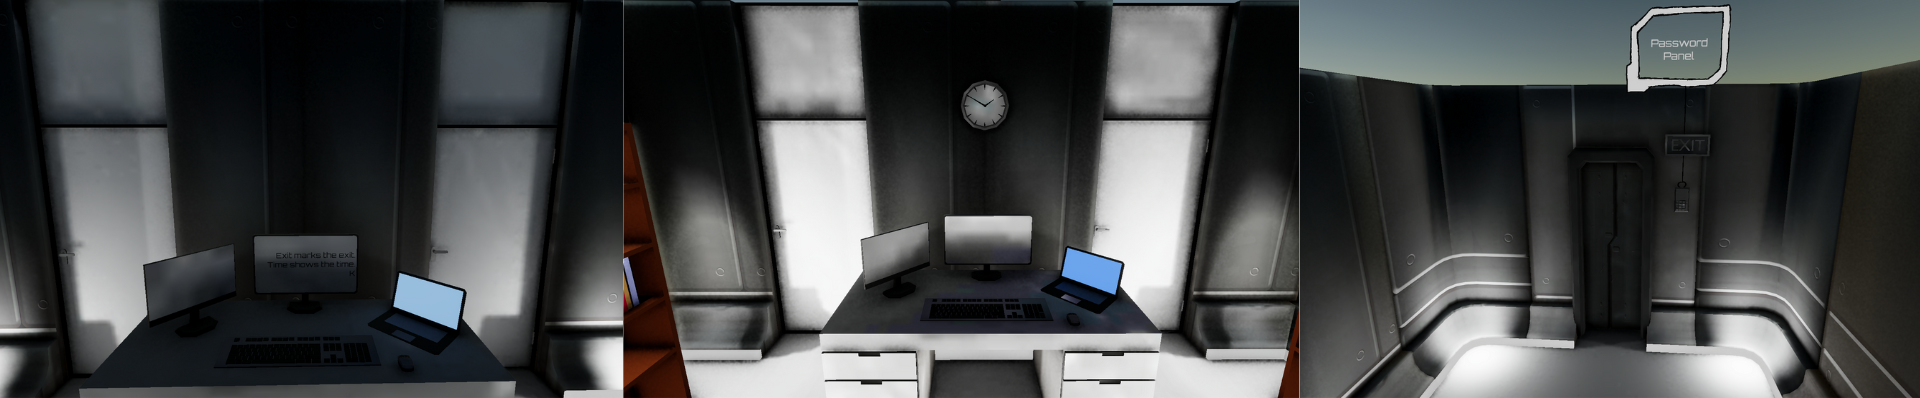
\includegraphics[width=1\linewidth]{content/pictures/Rätseldesign - Abschnitt02 - Rätsel04.png}
\caption{Aufbau der Rätsel von Abschnitt 3, Teil 5 (Quelle: eigene Darstellung)}
\label{fig:riddle-design-section02-04}
\end{figure}

Nachdem der Player den neuen Korridor betreten hat, stößt er auf einige verschlossene Türen (vgl. Abbildung \ref{fig:riddle-design-section02-00}, Bild erste Reihe links). Zum Start muss der Player den Druckbefehl starten, welcher in der Watcher Anwendung am Laptop zu sehen ist (vgl. Abbildung \ref{fig:riddle-design-section02-00}, Bild zweite Reihe links). Wurde der Druckvorgang gestartet, erhält der Player eine Notiz mit der Zahlenkombination zur Küche (vgl. Abbildung \ref{fig:riddle-design-section02-00}, Bild zweite Reihe Mitte). Der Watcher sieht zu diesem Zeitpunkt bereits die Küche und muss den Player zu dieser  navigieren. In der Küche angekommen, entdeckt der Player einen Projektor und ein Buch. Diese Gegenstände werden zu späteren Rätseln gebraucht. (vgl. Abbildung \ref{fig:riddle-design-section02-00}, Bild zweite Reihe rechts). 

Sobald der Projektor entdeckt und auch beim Watcher angezeigt wurde, öffnet sich das Konferenzzimmer (vgl. Abbildung \ref{fig:riddle-design-section02-0l}, Bild erste Reihe Mitte und Bild erste Reihe Rechts). Der Player als auch der Watcher sehen Stühle im Innenbereich des großen Konferenzraums. Anzumerken ist hier, dass sich die Anzahl der Stühle jeweils in den Anwendungen entscheiden. So erscheinen beim Watcher alle Stühle, zusätzlich zu den bereits existierenden, nachdem der Player diese entdeckt hat (vgl. Abbildung \ref{fig:riddle-design-section02-0l}, Bild erste Reihe rechts und zweite Reihe links). Nachdem der Watcher den gefundenen Projektor auf den Tisch platziert, erscheint eine Nachricht auf der Leinwand und das Team muss weiter ins Badezimmer (der Spruch \say{The chamber has been opened} orientiert sich dabei an den Spruch der Kammer des Schreckens aus Harry Potter 2 und bezieht sich dabei auf das anliegende WC) (vgl. Abbildung \ref{fig:riddle-design-section02-0l}, Bild zweite Reihe Mitte und zweite Reihe rechts).

Im Badezimmer erhält der Player einen Hinweis darauf, was der Watcher mit den Stühlen im Konferenzzimmer machen muss. An den Türen der Toilettenkabinen befinden sich drei verschiedene Symbole (die Symbole wurden aus dem Spiel \say{We were here too} entnommen (vgl. \cite{noauthor_we_nodate})) die jeweils für die Anordnungen der Stühle stehen. Die Abbildungen der Anordnungen befinden sich auf den an der Wand hängenden Postern (vgl. Abbildung \ref{fig:riddle-design-section02-02}, Bild erste Reihe rechts und zweite Reihe links). Das richtige der drei Symbole kann der Watcher in der Küche entdecken. Es ist, wenn man die Küche betritt, auf der rechten Seite die Rückwand der Küche zum Flur. (vgl. Abbildung \ref{fig:riddle-design-section02-02}, Bild erste Reihe Mitte). Nachdem die Stühle vom Watcher erneut in der richtigen Anordnung platziert wurden, erscheint eine weitere Nachricht auf der Leinwand. \say{The chairs haven fallen} Diese Nachricht sagt dem Player, dass die Stühle richtig platziert wurden und sich nun ein weiterer Raum geöffnet hat (vgl. Abbildung \ref{fig:riddle-design-section02-02}, Bild zweite Reihe rechts).

Am linken Ende des Korridors hat sich nun ein kleines Büro geöffnet, zu dem der Player und Watcher nun Zugang haben (vgl. Abbildung \ref{content/pictures/Rätseldesign - Abschnitt02 - Rätsel03.png}, Bild erste Reihe links). Das Büro gibt es in zwei unterschiedlichen Versionen. Für den Player öffnet sich die Tür zum Büro, welches eben beschrieben wurde. Für den Watcher öffnet sich die Tür gegenüber dieser Tür. Die Räume sind fast identisch, jedoch fehlen beim Player ein paar Dinge, welche ergänzt werden müssen. Die Büroräume bestehen aus zwei kleinen Unterräumen. Der erste Raum dient als kleine Bibliothek, in dem ein Bücherregal steht (vgl. Abbildung \ref{fig:riddle-design-section02-03}, Bild erste Reihe Mitte). Der zweite Raum wird im nächsten Schritt erzählt. In der Anwendung des Watchers befinden sich alle Bücher in dem Bücherregal, auch die, die bei der Anwendung des Players fehlen (vgl. Abbildungen \ref{fig:riddle-design-section02-03}, Bild zweite Reihe rechts und erste Reihe rechts). Die fehlenden Bücher befinden sich in der Küche (vgl. Abbildung \ref{fig:riddle-design-section02-03}, Bild zweite Reihe links) und bei den Waschbecken im Badezimmer (vgl. Abbildung \ref{fig:riddle-design-section02-03}, Bild zweite Reihe Mitte). Werden die Bücher in der richtigen Reihenfolge eingesetzt (das graue Buch links und das hellblaue Buch rechts) öffnet sich die linke weiße Tür zum hinteren Teil des Büros (vgl. Abbildung \ref{fig:riddle-design-section02-03}, Bild erste Reihe Mitte).

Das hintere Teil des Büros ist dann der Arbeitsplatz innerhalb eines Büros. Hier befindet sich ein Schreibtisch mit einem Computer und Monitoren. Links und rechts an den Wänden befinden sich noch Bücherregale, die für das letzte Rätsel nicht wichtig sind. Betritt der Player den Raum, so kann er auf einem Monitor auf dem Schreibtisch eine Notiz lesen: \say{Exit marks the exit. Time shows the time. K.} (vgl. Abbildung \ref{fig:riddle-design-section02-04}, Bild links). Diese Notiz bezieht sich auf das Passwort des Ausganges. Außerdem wird in der Notiz darauf hingewiesen, wo der Ausgang zu finden ist.
Der hintere Teil des Büros wurde nun auch für den Watcher sichtbar. Im veränderten Büro sieht der Watcher keine Notiz, aber eine Uhr. Sie zeigt anhand ihrer Uhrzeit das Passwort für den Ausgang (vgl. Abbildung \ref{fig:riddle-design-section02-04}, Bild Mitte). Der Ausgang, der mit einem \say{Exit}-Schild markiert ist, befindet sich am rechten Ende des Korridors, neben der Tür zum Konferenzzimmer (vgl. Abbildung \ref{fig:riddle-design-section02-04}, Bild rechts und Abbildung \ref{fig:riddle-design-section02-0l}, Bild erste Reihe Mitte). Tippt der Player nun das richtige Passwort ein, ist das Tutorial erfolgreich beendet und Player als auch Watcher würden aus dem Teil des Bürokomplexes entkommen.

\section{Dialoge}
Das grundlegende Spielkonzept sieht einen Dialog vor, der den Spielenden mehr Hintergrundinformationen vermittelt und den aktuellen Spielfortschritt erklärt. Anders als in vielen anderen Spielen wird der Dialog jedoch nicht identisch für beide Anwendungen sein. Stattdessen werden die Dialoge so gestaltet, dass sich die Spielenden den Text gegenseitig vorlesen müssen. Ziel dieses Ansatzes ist es, die wechselseitige Kommunikation zu fördern und die Zusammenarbeit zwischen den Spielteillehmenden zu stärken.

\section{Sounddesign}
Das Sounddesign soll den visuellen Eindruck der jeweiligen Anwendung durch ein auditives Feedback unterstützen. Sowohl der Avatar des Players, also auch die Interaktionen des Watchers sollen dabei ein auditives Feedback erzeugen.

Außerdem erhalten jeweils der Player und Watcher über bestimmte Töne ein auditives Feedback dazu, dass sie einzelne Rätsel gelöst und neue Wege freigeschaltet wurden.

Die entsprechende Ausgestaltung des Sounddesign werden in den folgenden Unterkategorien beschrieben.

Allgemein wird das Sounddesign jedoch im Hintergrund belassen, da es sonst die Kommunikation der Spielteilnehmer stören würde.

\subsection{Hintergrundmusik}
Jedes einzelne Szenario besitzt eine eigene atmosphärische Hintergrundmusik, welche der Spielwelt als Untermalung dient. Sie bestimmt ebenfalls den Effekt der Geräusche, die der Avatar des Players und die Aktionen des Watchers verursachen. So haben Geräusche bspw. einen Hall-Effekt im leeren Bürokomplex, oder einen dumpfen Unterton im Verlies.

Das Haupt- und Pausemenü besitzen ebenfalls einen atmosphärische Untermalung. Diese ist zur Pause und Beruhigung gedacht, hat aber auch einen Bezug zum Setting des Spiels.

\subsection{Umgebungsgeräusche}
Jedes dynamische oder Licht gebende Weltobjekt erzeugt bei Interaktion, Platzierung oder Entfernung Geräusche, die je nach Umgebung einen anderen Hall haben. Schwere Gegenstände wie die Säule würden beim Platzieren und Entfernen ein Kratzen auf dem Boden erzeugen. 


\subsection{Interaktionsgeräusche}
Jedes Interaktion des Players kann Geräusche erzeugen, so würde das Tragen einer Fackel in der Kleidung ein Rascheln erzeugen oder aber das Einsetzen in die Halterung ein Holz-auf-Metall klacken. Sobald der Watcher in seinen Menüs Gegenstände platziert, erhält er für die Auswahl als auch für das bewegen der Objekte im Menü ein auditives Feedback. So würde er bei der Positionsauswahl ebenfalls ein Kratzen oder Schleifen der Objekte auditiv wahrnehmen.


\section{Weitere nicht berücksichtigte Überlegungen}
In diesem Kapitel werden verworfene Konzeptideen vorgestellt, die nicht in das fertige Konzept integriert werden konnten.

Aus dem zugrundelegenden Konzept ging hervor, dass mehrere Watcher in einer Session mit einem Player zusammen interagieren sollen. Aus diesem Grund wurden nach Rückfragen in der Abschlusspräsentation des vorangegangenen Projekts bezüglich der Anzahl der Watcher Überlegungen getroffen, wie  zB. verschiedene Watcher oder mehr als 2 Teilnehmer beschäftigt werden können, ohne dass sie sich gegenseitig behindern. Zunächst wurde überlegt, kleine Minispiele einzubauen, die man aus Spielen wie \say{Duskwood} (vgl. \cite{everbyte_duskwood_nodate}) oder \say{Sentence} (vgl. \cite{jaunt_sentence_nodate})was?????? Allerdings würde das  dem Spielkonzept und dem Fokus auf der Kommunikation der Teilnehmer keinen Mehrwert bringen. Zudem würde es zu sehr von der Hauptspielmechanik und den eigentlichen Aufgaben ablenken.

?????An der Idee von mehreren Teilnehmern setzt die folgende Idee von Teams, die innerhalb der Spielwelt konträre Aufgaben haben. Sie können so aussehen, als würde ein Team zusammen Hindernisse für das Player-Watcher Team errichten. Daraus würde
eher ein Wettbewerb entstehen und die zielgerichtete Zusammenarbeit würde dabei
in den Hintergrund rücken. ?????

In Bezug auf eine ausgeglichene Aufgabenverteilung der beiden Spielerrollen Player und Watcher wurden ebenfalls Ideen gesammelt, um ein ausgeglichenes Spielerlebnis zu erlangen. Um das Spielerlebniss des Watchers auszuweiten, wurde überlegt ob ein Crafting-System im Spielszenario Sinn ergeben würde. Der Player würde dabei verarbeitbare Gegenstände in der Spielwelt finden, welche der Watcher im Crafting-Menü zu leichten oder schweren Gegenständen zusammenbringen könnte. Diese neuen Gegenstände könnten für weitere Rätsel oder Hindernisse gebraucht werden. Aus dem Grund der Sinnhaftigkeit und dem zeitlichen Aufwand, die neuen Gegenstände zu gestalten und zu platzieren, wurde diese Idee in dem finalen Konzept außen vor gelassen. 

Eine weitere Idee, analog zum Crafting-System, wäre ein Notizsystem, welches im Spiel \say{Shadow of doubt} (vgl. \cite{colepowered_games_shadows_nodate}) beispielhaft eine Kernmechanik ist. Der Watcher würde auf einer Notiztafel vom Player gesammelte Notizen anheften und weitere erstellen können. Entweder würde er Screenshots von Ausschnitten der Spielwelt oder Textnotizen anlegen. Sie sollen dabei helfen, die Rätsel der Spielwelt zu entschlüsseln und planen, welche Rätsel im nächsten Schritt gelöst werden müssen. Zunächst ????oder wurde diese Funktion außen vor gelassen?????? wurde diese Funktion herausgelassen, da der Watcher weitere Funktionen wie das Drehen und Vergrößern von Gegenständen im Verlauf des Spiels erhält, aber auch weil die Rätsel und Hindernisse oft nur durch das Platzieren von Gegenständen gelöst werden können und für ein umfangreicheres Rätseldesign ein höherer Zeitaufwand nötig gewesen wäre.

% [custom events für verschiedene Watcher, dass die so zwischewnaufgaben haben wie bei den story driven handy games]

% [Einbauen von Gegner teams für den Team-work aspekt -> hat zur folge dass mehr teilnehmer benötigt werden]

% [Craftsystem beim Watcher für mehr Aufgaben]
% [Notizsystem wie bei shadow of doubts für mehr aufgaben]

% [Fähig]


% \section{Rollenspezifisches Design}

% \section{Genre}

% \section{Spielmechanik}

% \section{Spielablauf}

% \subsection{Spielablauf des Spiels}

% \subsection{Levelablauf}

% \section{Session}

% % \section{Belohnungen}

% \section{Spielerrollen}

% \subsection{Player}

% % \subsubsection{Interaktion mit Gegenständen}

% % \subsubsection{Tragen von Gegenständen}

% \subsection{Watcher}

% % \subsubsection{Platzieren von Gegenständen}

% % \subsubsection{Entfernen von Gegenständen}

% % \subsubsection{Previewen von Gegenständen}

% \section{Gegenstände}

% \subsection{Leichte Gegenstände}

% \subsection{Schwere Gegenstände}

% \subsection{Hinweise}

% \section{Leveldesign}

% \subsection{Gegenstände}

% \subsection{Hinweise}

% \subsection{Hindernisse}

% \section{Informationen für den Spieler}

% \section{Sounddesign}

% \chapter{Visuelles Design des Prototyps}

% \section{Moodboard}

% \section{Art-Stil}

% \section{Avatar des Players}

% \section{User Interface}

% \section{Führung durch das Level}

% \section{Gegenstände}

% \section{Menü}

% \section{Leveldesign}